% Format teze zasnovan je na paketu memoir
% http://tug.ctan.org/macros/latex/contrib/memoir/memman.pdf ili
% http://texdoc.net/texmf-dist/doc/latex/memoir/memman.pdf
% 
% Prilikom zadavanja klase memoir, navedenim opcijama se podešava 
% veličina slova (12pt) i jednostrano štampanje (oneside).
% Ove parametre možete menjati samo ako pravite nezvanične verzije
% mastera za privatnu upotrebu (na primer, u b5 varijanti ima smisla 
% smanjiti 
\documentclass[12pt,oneside]{memoir} 

% Paket koji definiše sve specifičnosti master rada Matematičkog fakulteta
\usepackage[latinica]{matfmaster} 

\usepackage[bottom]{footmisc}
\usepackage{latexsym}
\usepackage{amssymb}
\usepackage{amsmath}
\usepackage{algorithm}
\usepackage{algpseudocode}
\usepackage{listings}
\usepackage{bm}
\usepackage{multirow}

\usepackage{array}
\newcolumntype{P}[1]{>{\centering\arraybackslash}p{#1}}
\usepackage{float}


% Define a custom color
\definecolor{backcolour}{rgb}{0.95,0.95,0.92}
\definecolor{codegreen}{rgb}{0,0.6,0}

% Define a custom style
\lstdefinestyle{myStyle}{
    backgroundcolor=\color{backcolour},   
    commentstyle=\color{codegreen},
    basicstyle=\ttfamily\footnotesize,
    breakatwhitespace=false,         
    breaklines=true,                 
    keepspaces=true,                 
    numbers=left,       
    numbersep=5pt,                  
    showspaces=false,                
    showstringspaces=false,
    showtabs=false,                  
    tabsize=2,
}

% Use \lstset to make myStyle the global default
\lstset{style=myStyle}

\makeatletter
\renewcommand{\ALG@name}{Algoritam}
\makeatother
%
% Podrazumevano pismo je ćirilica.
%   Ako koristite pdflatex, a ne xetex, sav latinički tekst na srpskom jeziku
%   treba biti okružen sa \lat{...} ili \begin{latinica}...\end{latinica}.
%
% Opicija [latinica]:
%   ako želite da pišete latiniciom, dodajte opciju "latinica" tj.
%   prethodni paket uključite pomoću: \usepackage[latinica]{matfmaster}.
%   Ako koristite pdflatex, a ne xetex, sav ćirilički tekst treba biti
%   okružen sa \cir{...} ili \begin{cirilica}...\end{cirilica}.
%
% Opcija [biblatex]:
%   ako želite da koristite reference na više jezika i umesto paketa
%   bibtex da koristite BibLaTeX/Biber, dodajte opciju "biblatex" tj.
%   prethodni paket uključite pomoću: \usepackage[biblatex]{matfmaster}
%
% Opcija [b5paper]:
%   ako želite da napravite verziju teze u manjem (b5) formatu, navedite
%   opciju "b5paper", tj. prethodni paket uključite pomoću: 
%   \usepackage[b5paper]{matfmaster}. Tada ima smisla razmisliti o promeni
%   veličine slova (izmenom opcije 12pt na 11pt u \documentclass{memoir}).
%
% Naravno, opcije je moguće kombinovati.
% Npr. \usepackage[b5paper,biblatex]{matfmaster}

% Pomoćni paket koji generiše nasumičan tekst u kojem se javljaju sva slova
% azbuke (nema potrebe koristiti ovo u pravim disertacijama)
\usepackage[latinica]{pangrami}

% Datoteka sa literaturom u BibTex tj. BibLaTeX/Biber formatu
\bib{matfmaster-primer}

% Ime kandidata na srpskom jeziku (u odabranom pismu)
\autor{Miloš P. Miković}
% Naslov teze na srpskom jeziku (u odabranom pismu)
\naslov{Algoritmi za rešavanje problema najkraće zajedničke nadniske}
% Godina u kojoj je teza predana komisiji
\godina{2021}
% Ime i afilijacija mentora (u odabranom pismu)
\mentor{dr Aleksandar \textsc{Kartelj}, docent\\ Univerzitet u Beogradu, Matematički fakultet}
% Ime i afilijacija prvog člana komisije (u odabranom pismu)
\komisijaA{dr Vladimir \textsc{Filipović}, redovni profesor\\ Univerzitet u Beogradu, Matematički fakultet}
% Ime i afilijacija drugog člana komisije (u odabranom pismu)
\komisijaB{dr Stefan \textsc{Mišković}, docent\\ Univerzitet u Beogradu, Matematički fakultet}
% Ime i afilijacija trećeg člana komisije (opciono)
% \komisijaC{}
% Ime i afilijacija četvrtog člana komisije (opciono)
% \komisijaD{}
% Datum odbrane (odkomentarisati narednu liniju i upisati datum odbrane ako je poznat)
% \datumodbrane{}

% Apstrakt na srpskom jeziku (u odabranom pismu)
\apstr{%
% \pangrami
Problem najkraće zajedničke nadniske predstavlja jedan od dobro poznatih i ispitivanih
NP-teških problema optimizacije. Zbog njegove široke primene u mnogim oblastima informatike,
na njegovom što efikasnijem rešenju radi se poslednje četiri decenije.
Vremenom je predloženo mnoštvo algoritama koji kombinuju različite optimizacione
tehnike i pristupe. U ovom radu predstavljena su dva algoritma koji rešavaju
ovaj problem. Algoritam grananja sa odsecanjem uvek pronalazi optimalno rešenje
problema ali je njegovo vreme izvršavanja u najgorem slučaju eksponencijalno.
Drugi predstavljeni algoritam počiva na metaheurističkoj tehnici
pretraga bima (\textit{eng.} beam search) u kombinaciji sa dve pohlepne
heurističke funkcije većinsko spajanje (\textit{eng.} majority merge)
i težinsko većinsko spajanje (\textit{eng.} weighted majority merge).
U radu je detaljno opisan problem i konstrukcija pomenutih algoritama i heurističkih funkcija.
Opisan je način na koji su generisane test instance problema i dat je prikaz
rezultata na različitim instancama problema. Ukratko su opisane već korišćene tehnike
za rešavanje ovog problema i date ideje za pravce daljeg usavršavanja predstavljenog algoritma
ili formiranje novog.
}

% Ključne reči na srpskom jeziku (u odabranom pismu)
\kljucnereci{optimizacija, pretraga bima, analiza bioloških sekvenci, zajednička nadniska,
težinsko spajanje, većinsko težinsko spajanje}

\begin{document}
% ==============================================================================
% Uvodni deo teze
\frontmatter
% ==============================================================================
% Naslovna strana
\naslovna
% Strana sa podacima o mentoru i članovima komisije
\komisija
% Strana sa posvetom (u odabranom pismu)
\posveta{Hvala profesoru Aleksandru Kartelju.}
% Strana sa podacima o disertaciji na srpskom jeziku
\apstrakt
% Sadržaj teze
\tableofcontents*

% ==============================================================================
% Glavni deo teze
\mainmatter
% ==============================================================================

% ------------------------------------------------------------------------------
\chapter{Uvod}
\label{chap:uvod}
% ------------------------------------------------------------------------------
% \pangrami
Problem najkraće zajedničke nadniske (\textit{eng.} Shortest Common Supersequence Problem)
jedan je od dobro poznatih NP-teških problema optimizacije u oblasti analize reči \cite{ProbabilisticBS}.
Ukratko, PNZN\footnote{U nastavku teksta PNZN ćemo koristiti kao skraćenicu za problem najkraće zajedničke nadniske}
se može opisati kao problem pronalaženja najkraće reči $\omega$ sačinjene
od simbola zadate konačne Azbuke $\Sigma$, tako da su sve sekvence iz unapred zadatog konačnog skupa
$\mathcal{L}$ sadržane u sekvenci $\omega$. Kada se kaže da su sve reči iz skupa $\mathcal{L}$
sadržane, misli se na to da se svaka reč iz skupa $\mathcal{L}$ može dobiti uklanjanjem simbola iz reči $\omega$ ali 
u zadatom redosledu \cite{SCSSProblemDef}. PNZN ima primene u mnogim oblastima informatike uključujući kompresiju podataka
\cite{DataCompression}, optimizaciju upita \cite{MQOptimization}, analizu i poređenje teksta i bioloških sekvenci, \cite{ITAlgorithms} \cite{SeqComparison}
kao i bioinformatiku \cite{ProbabilisticBS}.
Kao rezultat velike primene u mnogim oblastima, postoji veliki broj istraživanja na temu ovog problema u pokušaju da se dođe
do što boljeg i prihvatljivijeg rešenja. Trenutno najbolji algoritmi za rešavanje PNZN počivaju na metaheurističkoj metodi
pretraga bima (\textit{eng.} beam search) koja će biti predstavljena u ovom radu. U nastavku uvodnog poglavlja biće formalno
definisan problem najkraće zajedničke nadniske i biće dat pregled dosadašnjih istraživanja na temu ovog problema.

\section{Problem najkraće zajedničke nadniske}
U ovom poglavlju formalno ćemo definisati PNZN, ali pre toga uvešćemo potrebnu notaciju koja će biti korišćena u nastavku
teksta. Konačna azbuku sastoji se od konačnog broja slova i označavaćemo je sa $\Sigma$. Svaka konačna reč
$\omega=\omega(1)\omega(2)...\omega(n)$ sastoji se od konačnog broja slova azbuke gde $\omega(j)\in\Sigma$ predstavlja j-to slovo reči $\omega\in\Sigma^*$.
Duzinu reči $\omega$ označavaćemo sa $|\omega|$, praznu reč sa $\varepsilon$ i važi da $|\varepsilon|=0$. 
% U skladu sa uvedenom
% notacijom $|\Sigma|$ predstavlja kardinalnost azbuke. Sa $\omega\unrhd\alpha$ označavaćemo broj pojavljivanja slova $\alpha$
% u reči $\omega$ ($\omega(1)\omega(2)...\omega(n)\unrhd\alpha=\sum_{1<=i<=n,\omega(i)=\alpha}1$). 
Reč koja se dobija dodavanjem
slova $\alpha$ na početak reči $\omega$ označavaćemo sa $\alpha\omega$,
%  (takođe ćemo pisati $\omega=\alpha\omega^{'}$),
a reč koja se dobija dodavanjem slova $\alpha$ na kraj reči $\omega$ sa $\omega\alpha$
% , slično reč koja se dobija skidanjem slova $\alpha$ sa početka
% reči $\omega$ sa $\omega|_{\alpha}$. 
% Brisanje slova $\alpha$ sa početka svake reči u zadatom skupu, u skladu sa uvedenom notacijom
% definišemo kao $\{\omega_{1},\omega_{2},...,\omega_{n}\}|_{\alpha}=\{\omega_{1}|_{\alpha},\omega_{2}|_{\alpha},...,\omega_{n}|_{\alpha}\}$.
Sa $\omega[a:b]$\footnote{Slično kao indeksiranje nizova u programskom jeziku Python} označavaćemo reč koja se dobija od
reči $\omega$ počevši od pozicije $a$ do pozicije $b$ u reči $\omega$. Ako se izostavi vrednost pozicije $a$, podrazumeva se
da je početna pozicija 0, slično ako se izostavi vrednost pozicije $b$ podrazumeva se vrednost $m-1$ ako $|\omega|=m$.
Na primer $\omega[:]$ predstavlja samu reč $\omega$. Pristupanje slovu na poziciji $i$ reči $\omega$ 
označavaćemo sa $\omega[i]$.

Neka važi da $\omega_{1},\omega_{2}\in\Sigma^*$, za reč $\omega_{1}$ kažemo da je
supersekvenca reči $\omega_{2}$ u oznaci $\omega_{1}\succ\omega_{2}$ ako važi sledeća rekurzivna definicija \cite{ProbabilisticBS}:
\\
\\
\begin{equation}
\begin{aligned}
\omega_{1}\succ\varepsilon &\triangleq \textrm{Tačno}\\
\varepsilon\succ\omega_{2} &\triangleq \textrm{Netačno, \:\:Ako } \omega_{2}\neq\varepsilon\\
\alpha\omega_{1}\succ\alpha\omega_{2} &\triangleq \omega_{1}\succ\omega_{2}\\
\alpha\omega_{1}\succ\beta\omega_{2} &\triangleq \omega_{1}\succ\beta\omega_{2} \textrm{, \:\:Ako } \alpha\neq\beta
\end{aligned}
\end{equation}
\\

Zapravo, $\omega_{1}\succ\omega_{2}$ označava da se svi simboli iz $\omega_{2}$ nalaze u $\omega_{1}$ u datom redosledu,
ali ne nužno uzastopno. Na primer, za datu azbuku $\Sigma=\{a,c,t,g\}$, važi $agcatg \succ act$.
Sada možemo formalno definisati PNZN. Instanca PNZN može se definisati kao $\mathcal{I} =(\Sigma,\mathcal{L})$, gde 
$\Sigma$  predstavlja konačnu azbuku, a $\mathcal{L}$ predstavlja skup od $m$ reči $\{\omega_{1},\omega_{2},...,\omega_{m}\}$,
$\omega_{i}\in\Sigma^*$. Potrebno je pronaći reč $\omega$ najmanje dužine tako da važi da je $\omega$ supersekvenca svake reči iz
skupa $\mathcal{L}$ ($\omega\succ\omega_{i}, \forall\omega_{i}\in\mathcal{L} \textrm{ i } |\omega| \textrm{ je minimalna}$).
Na primer za instancu PNZN $\mathcal{I}=(\{a,c,t,g\},\{act,cta,aca\})$, najmanja zajednička supersekvenca
instance $\mathcal{I}$ je $acta$.

Može se pokazati da je PNZN NP-težak problem, čak i ako su jaka ograničenja postavljena na $\mathcal{L}$ ili $\Sigma$. 
Dokazano je da je PNZN NP-kompletan problem nad svakom azbukom $\Sigma$ za koju važi da $|\Sigma|\geqslant2$ \cite{NPComplete}
ili kada su sve reči $\omega \in \mathcal{L}$ dužine dva \cite{SCSNP}. U principu ovim rezultatima NP-težine se mora
pristupiti sa oprezom, jer predstavljaju samo najgori scenario što često u praksi nije slučaj. U odnosu na to,
realnija karakterizacija težine može se dobiti korišćenjem okvira parametrizovane složenosti (\textit{eng.} framework of parameterized
complexity). Ukratko, ovo se postiže višedimenzionim pristupom problemu, shvatanjem njegove unutrašnje strukture i izolovanjem
određenih parametara. Ako se težina (koja nije polinomijalna) može izolovati unutar ovih parametara, problem može biti
efikasno rešen za fiksne vrednosti ovih parametara. Na primer može se uzeti
maksimalna dužina $k$ nadniske kao parametar i ako je pritom veličina azbuke fiksna ili parametar takođe, problem postaje
fiksno-parametarski pratljiv (\textit{eng.} fixed-parameter tractable) jer postoji maksimalno $|\Sigma|^{k}$ nadniski
koje se mogu proveriti kao rešenje problema \cite{ProbabilisticBS}. Može se parametrizovati i broj reči u skupu $\mathcal{L}$.

\section{Pregled dosadašnjih istraživanja}
Problem najkraće zajedničke nadniske prvi je uveo Dejvid Mejer (\textit{eng.} David Maier) 1978. godine u svom radu 
"The Complexity of Some Problems on Subsequences and Supersequences" \cite{Maier}. Korišćenjem dinamičkog
programiranja (\textit{eng.} dynamic programming) PNZN nad dve reči dužine $n$ rešen je algoritmom vremenske 
složenosti $\mathcal{O}(n^{2})$ i prostorne složenosti $\mathcal{O}(n^{2})$. Algortiam zasnovan na dinamičkom programiranju
može biti unapređen, pa tako za $k$ reči dužine maksimalno $n$, PNZN može biti rešen u $\mathcal{O}(n^{k})$ prostornoj i 
vremenskoj složenosti \cite{SCSDinamicProg}. Jasno je da ovakav algoritam nije praktičan za velike vrednosti $k$. S obzirom na to da ne postoji 
algoritam polinomijalne složenosti koji rešava PNZN, pribegava se optimizacionim metodama u rešavanju ovog problema.
Ono što je karakteristično za optimizacioni pristup rešavanju problema jeste to da se formira algoritam koji rešava
postojeći problem tako što daje rešenje koje je prihvatljivo pod određenim uslovima. Takvo rešenje ne mora nužno biti
optimalno rešenje problem. Na ovaj način, korišćenjem određene optimizacione tehnike, dobija se algoritam koji se izvršava
brzo u realnim uslovima i daje prihvatljivo dobra rešenja.

Vremenom je predloženo mnogo heurističkih i metaheurističkih algoritama za rešavanje PNZN.
Neke od poznatijih heurističkih funkcija koje su korišćene u rešavanju PNZN su Alfabet (\textit{eng.} Alphabet) \cite{AlphabetSCS}, Većinsko Spajanje (\textit{eng.} Majority Merge) 
i Težinsko Većinsko Spajanje (\textit{eng.} Weighted Majority Merge) \cite{ProbabilisticBS}, Turnirska (\textit{eng.} Tournament) i Pohlepna (\textit{eng.} Greedy) \cite{Tournament},
Redukuj-Proširi (\textit{eng.} Reduce-Expand) \cite{AlphabetSCS}. Pored navedenih funkcija, korišćeni su i metaheuristički algoritmi, genetski algoritam (\textit{eng.} genetic algorithm) \cite{SCSGenetic} i 
optimizacija kolonijom (\textit{eng.} colony optimization) \cite{SCSColony}, koji predstavljaju složenije optimizacione tehnike i imaju
tendenciju ka dužem vremenu izvršavanja ne većim instancama problema \cite{SCSSBetterSolution}.

Jedna od trenutno najboljih metaheuristika za rešavanje PNZN jeste pretraga bima (\textit{eng.} beam search). Ukratko, pretraga
bima predstavlja nepotpunu pretragu stabla, koja na svakom nivou proširuje graf stanja tako što napreduje sa čvorovima koji najviše
obećavaju \cite{SCSBS}. Upravo zbog toga što se dobro pokazala u rešavanju PNZN i sličnih problema poput problema najduže zajedničke podniske
(\textit{eng.} longest common subsequence) pretraga bima će biti korišćena u ovom radu i biće detaljnije opisana u daljem tekstu.
S obzirom na to da pretraga bima podrazumeva postojanje heurističke funkcije koja će oceniti kvalitet čvorova na određenom nivou,
u ovom radu izabrane su dve takve funkcije, Većinsko Spajanje (\textit{eng.} Majority Merge) i Težinsko Većinsko Spajanje
(\textit{eng.} Weighted Majority Merge) koje su se dobro pokazale u prethodnim istraživanjima i one će detaljnije biti 
opisane u nastavku teksta.

% % Primeri citiranja\mathsf{Y} 
% Ovo je rečenica u kojoj se javlja citat \cite{PetrovicMikic2015}.
% Još jedan citat \cite{GuSh:243}.
% % Primeri navodnika
% Isprobavamo navodnike: "Rekao je da mu se javimo sutra".
% % Primer referisanja na tabelu (koja se javlja kasnije)
% U tabeli \ref{tbl:rezultati} koja sledi prikazani su rezultati eksperimenta.
% % Primer kraćeg ćiriličkog teksta
% {\cir Ово је пример ћириличког текста који се јавља у латиничком документу.}
% U ovoj rečenici se javlja jedna reč na {\cir ћирилици}.
% % Primer korišćenja fusnota
% % Iza ove rečenice sledi fusnota.\footnote{Ovo je fusnota.}

% % Primer dužeg ćirličkog teksta
% \begin{cirilica}
%   Ово је мало дужи блок текста исписан ћириличким писмом у оквиру
%   латиничког документа. Фијуче ветар у шибљу, леди пасаже и куће иза
%   њих и гунђа у оџацима.
% \end{cirilica}

% % Primer korišćenja tabele
% \begin{table}
% \centering
% \caption{Rezultati}
% \label{tbl:rezultati}
% \begin{tabular}{c>{\centering}p{2cm}c}
% \toprule
% 1 & 2 & 3\\\midrule
% 4 & 5 & 6\\\cmidrule(rl){1-2}
% 7 & 8 & 8\\
% \bottomrule
% \end{tabular}
% \end{table}

% % Primer korišćenja slike
% \begin{figure}[!ht]
%   \centering
%   \label{fig:grafikon}
%   
\includegraphics[width=0.5\textwidth]{graph.png}
%   \caption{Grafikon}
% \end{figure}


% % Primer jednostavnije matematičke formule
% Evo i jedan primer matematičke formule: $e^{i\pi} + 1 = 0$. 
% % Primer referisanja na sliku
% Na slici \ref{fig:grafikon} prikazan je jedan grafikon.

% % primer kompleksnije matematičke formule
% $$
% \int_a^b f(x)\ \mathrm{d}x \ =_{def}\ \lim_{\max{\Delta x_k \rightarrow 0}} \sum_{k=1}^n f(x_k^*)\Delta x_k
% $$

% % primer referisanja na poglavlja i strane poglavlja
% Više detalja biće dato u glavi \ref{chp:razrada} na strani \pageref{chp:razrada}.

% % primer liste
% Možemo praviti i nabrajanja:
% \begin{enumerate}
% \item Analiza 1
% \item Linearna algebra
% \item Analitička geometrija
% \item Osnovi programiranja
% \end{enumerate}

% \pangrami

% ------------------------------------------------------------------------------
% \chapter{Opis korišćenih optimizacionih metoda}
% \label{chp:opisMetoda}

% % ------------------------------------------------------------------------------

% % \pangrami

% % \pangrami

% % ------------------------------------------------------------------------------
% U ovom poglavlju biće dat kratak pregled optimizacionih metoda koje su korišćene za rešavanje problema najkraće
% zajedničke nadniske. Te medote su:
% \begin{enumerate}
%   \item Metaheuristika Pretraga Bima
%   \item Heuristička funkcija Većinsko Spajanje
%   \item Heuristička funkcija Težinsko Većinsko Spajanje
% \end{enumerate}
% U nastavku teksta biće opisane pomenute metode, ali samo kao nezavisne celine, algoritam koji kombinuje
% rad ovih metoda biće predstavljen u narednom poglavlju.

% \section{Metaheuristika Pretraga Bima}
% \label{sec:pretragaBima}
% \begin{figure}[!ht]
%   \centering
%   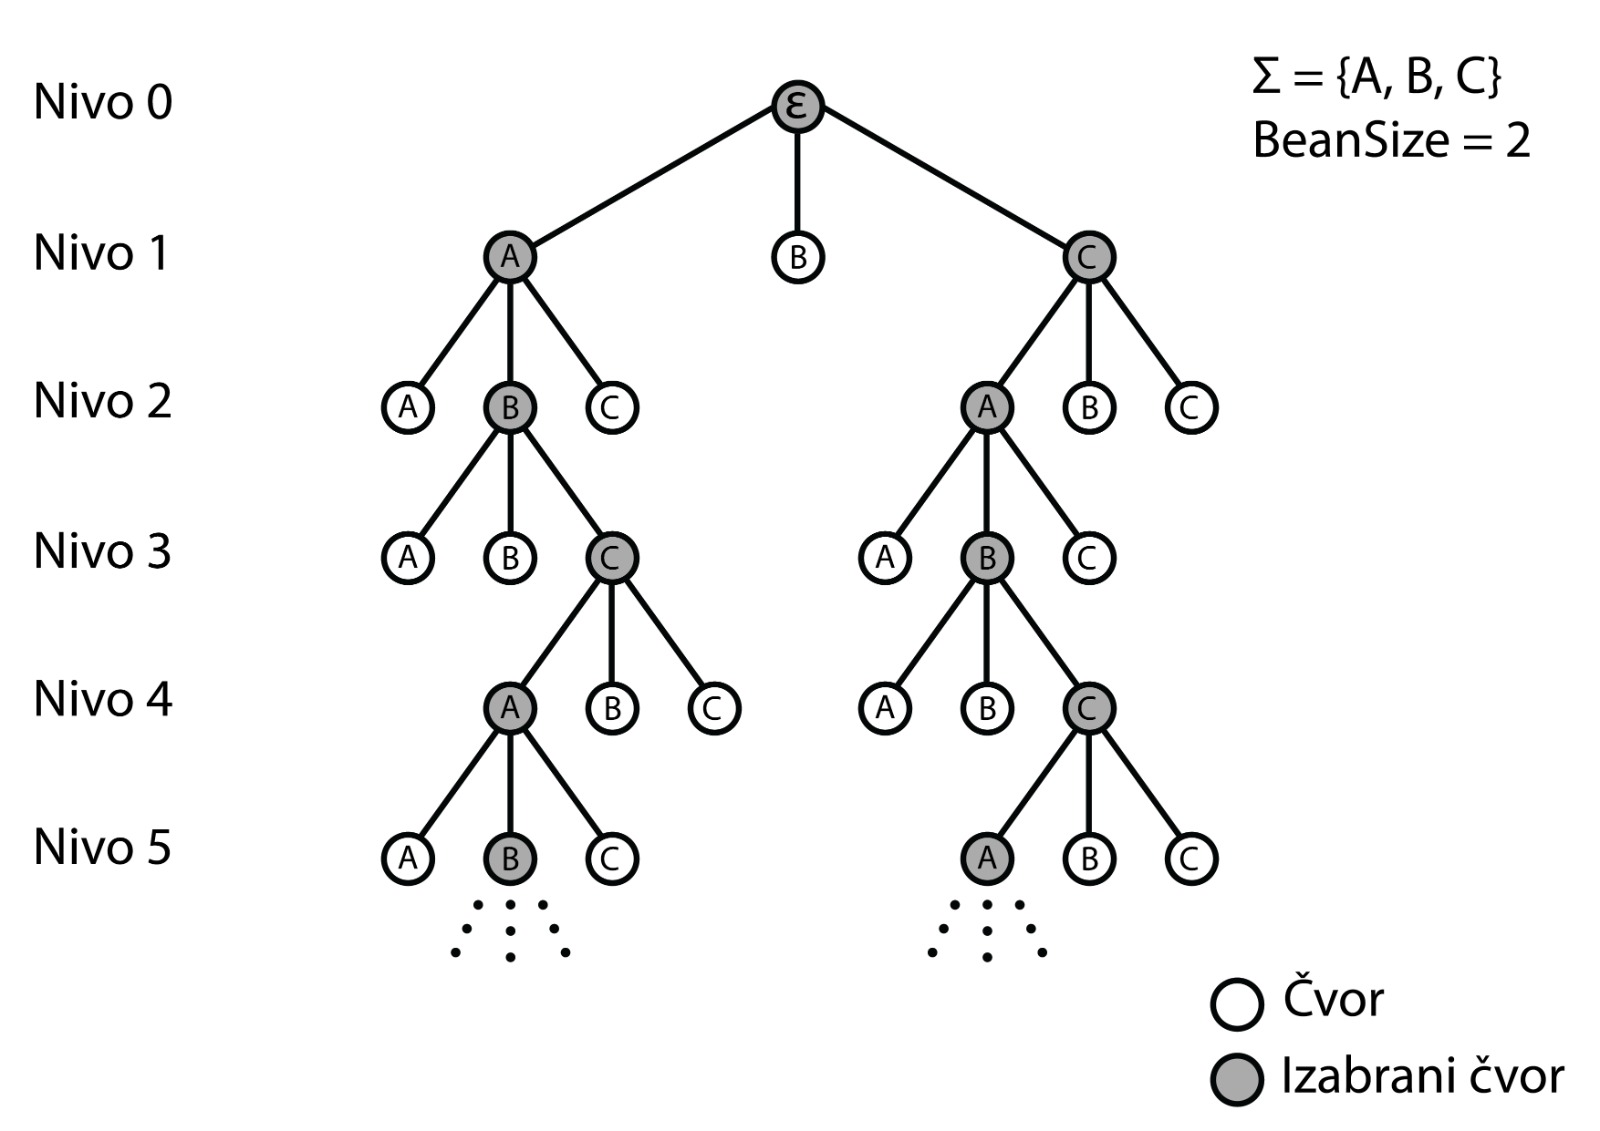
\includegraphics[width=1\textwidth]{Slike/bs2.png}
%   \caption{Šema metaheuristike Pretraga Bima} 
%   \label{fig:pretragaBima}
% \end{figure}
% Sada ćemo predstaviti generalnu ideju Pretrage Bima na kojoj ćemo kasnije izgraditi algoritam za PNZN.
% Pretraga Bima predstavlja metaheuristiku koja je uvedena 1976. godine u oblasti prepoznavanja govora
% (\textit{eng.} speech recognition). Korišćena je u završnim slojevima mnogih modela za
% obradu prirodnog jezika (\textit{eng.} natural language processing models) u donošenju odluke da se izabere najbolji
% izlaz date ciljne promenjive \cite{BSIntroduction}. Pored navedenih primena pretraga bima se intenzivno koristi u sledećeim
% oblastima: kombinatorna optimizacija (\textit{eng.} combinatorial optimization), problemi planiranja (\textit{eng.} scheduling problems),
% problemi rutiranja vozila (\textit{eng.} vehicle routing problems), podešavanje hiperparametara u oblasti mašinskog učenja
% (\textit{eng.} Machine Learning Hyperparameter Tuning), problemi zadovoljenja ograničenja (\textit{eng.} Constraint Satisfaction Problems). 

% Pretraga Bima predstavlja vrstu pretrage grafa u širinu u cilju da
% se pronađe najbolji put od korenog čvora do ciljanog čvora u grafu. Kako bi se složenost izračunavanja držala u
% zadatim granicama, Pretraga Bima evaluira dostignute čvorove na određenom nivou ali bira samo podskup od $\beta$
% čvorova koji najviše obećavaju i sa tim podskupom čvorova napreduje dalje u pretrazi. Izabrani podskup od $\beta$ čvorova
% zvaćemo bim (\textit{eng.} beam) i označavaćemo ga sa $\mathbb{B}$, a $\beta$ parametar ćemo zvati širina bima (\textit{eng.} beam width) \cite{SCSBS}.
% U kontekstu PNZN graf koji pretražujemo $\mathcal{G}=(\mathcal{V},\mathbb{E})$ predstavlja usmeren aciklički graf, a  
% pseudo kod algoritma prikazan je pod Algoritam \ref{alg:bs} i dat u kontekstu problema najkraće
% zajedničke nadniske. 
% \\
% \begin{algorithm}
%   \caption{PretragaBimaPNZN($\Sigma$, $\mathcal{L}$, $\beta$)}
%   \label{alg:bs}
%   \begin{algorithmic}[1]
%   % \Require $n \geq 0$
%   % \Ensure $y = x^n$
%   \State $\mathcal{B} \gets \{ \}$
%   \While{$\textrm{Tačno}$} \Comment{Može postojati uslov izlaska iz petlje pre pronađenog rešenja}
%   \State $\mathcal{B} \gets \textrm{ProširiBim}(\Sigma)$
%   \State $\textrm{OceniBim}(\mathcal{B}, \mathcal{L})$
%   \State $\mathcal{B} \gets \textrm{RedukujBim}(\mathcal{B}, \beta)$
%   % \State \If{x}
%   % \ElsIf{$N$ is odd}
%   \For{$\omega\in\mathcal{B}$}
%     \If{$\textrm{ZajedničkaNadniska}(\omega,\mathcal{L})$}
%     \State \Return $\omega$
%     \EndIf
%   \EndFor
%   \EndWhile
%   \end{algorithmic}
%   \end{algorithm}
% \\
% Algoritam prima tri ulazna parametra: azbuku $\Sigma$, ulazni skup reči $\mathcal{L}$ i širinu bima $\beta$.
% Na početku bim $\mathcal{B}$ predstavlja prazan skup. U svakom koraku algoritma bim se proširuje slovima iz azbuke,
% a zatim se elementi proširenog bima ocenjuje izabranom heurističkom funkcijom. Zatim se vrši odabir $\beta$ čvorova
% sa kojima se dalje nastavlja pretraga, i vrši se provera da li neki čvor u bimu predstavlja rešenje problema,
% ako takav čvor postoji algoritam vraća pronađeno rešenje. Funkcija ProširiBim u prvom koraku popunjava bim slovima
% iz azbuke, a u svakom narednom koraku svako parcijalno rešenje redukovanog bima proširuje dodavajući na njega redom
% slova iz azbuke. Funkcija OceniBim predstavlja heurističku funkciju koja dodeljuje određene vrednosti svakom elementu bima,
% a na osnovu ovih vrednosti funkcija RedukujBim bira $\beta$ parcijalnih rešenja koja imaju najveće vrednosti
% heurističke funkcije. Tokom redukcije bima vrednosti ocena parcijalnih rešenja mogu da se sortiraju tako da redukovani
% bim sadrži $\beta$ najbolje ocenjenih rešenja, ali mogu se koristiti i druge strategije odabira rešenja poput ruletske
% selekcije (\textit{eng.} roulette selection). Funkcija ZajedničkaNadniska vrši proveru da li reč $\omega$
% predstavlja zajedničku nadnisku reči iz skupa $\mathcal{L}$ i jedna njena implementacija će biti opisana u sledećem poglavlju.
% Algoritam se može zaustaviti kada se pronađe prvo rešenje problema, ali mogu se postaviti i drugi uslovi zaustavljanja
% poput broja iteracija petlje (predstavlja dubinu unutar stabla pretrage) ili vremenska ograničenja.

% \section{Heurističke funkcije Većinsko Spajanje i Težinsko Većinsko Spajanje}
% \label{sec:MMiWMM}
% Većinsko Spajanje predstavlja jedan od najpopularnijih algoritama koji rešava PNZN. To je pohlepni algoritam
% koji inkrementalno konstruiše supersekvencu. Najpre se odredi slovo koje se najčešće nalazi na početku reči
% iz skupa $\mathcal{L}$, a zatim se izabrano slovo briše sa početka reči iz $\mathcal{L}$ koje ga sadrže \cite{ProbabilisticBS}.
% Pseudo kod algoritma prikazan je pod Algoritam \ref{alg:mm}.

% \begin{algorithm}
%   \caption{VećinskoSpajanje($\mathcal{L}=\{\omega_{1}, \omega_{2},..., \omega_{m}\}, \Sigma$)}
%   \label{alg:mm}
%   \begin{algorithmic}[1]
%   % \Require $n \geq 0$
%   % \Ensure $y = x^n$
%   \State $\mathcal{S} \gets \varepsilon$ \Comment{supersekvenca}
%   \While{$\sum_{\omega_{i}\in\mathcal{L}}|\omega_{i}| \neq 0$} 
%   \For{$\alpha \in \Sigma$}
%         \State $v(\alpha|\mathcal{S}) \gets \sum_{\omega_{i}\in\mathcal{L},\omega_{i}=\alpha\omega^{'}_{i}}1$
%   \EndFor
%   \State $\beta \gets argmax \{v(\alpha|\mathcal{S})\textrm{ }|\textrm{ }\alpha \in \Sigma \}$
%   \State $\mathcal{L} \gets \mathcal{L}|_{\beta}$
%   \State $\mathcal{S} \gets \mathcal{S}\beta$
%   \EndWhile
%   \State \Return $\mathcal{S}$
%   \end{algorithmic}
%   \end{algorithm}

% Mana Većinskog Spajanja je to što ne može da prepozna globalnu strukturu reči iz skupa $\mathcal{L}$.
% U principu Većinsko spajanje izostavlja činjenicu da reči mogu biti različitih dužina. To dalje 
% znači da će slova sa početka kraćih reči imati veću šansu da budu uklonjena iako algoritam i dalje treba
% da obradi preostale dugačke reči. Iz tog razloga bi skidanje slova sa početka kraćih reči trebalo da bude
% manje prioritetno. Drugim rečima bolje je da se prioritizira skidanje slova sa početka dužih reči.
% To se može postići dodavanjem težine svakom simbolu azbuke u odnosu na dužinu preostalih reči iz $\mathcal{L}$ 
% nakon uklanjanja tog simbola sa početka reči koje počinju tim simbolom. Dakle korak 4 u algoritmu VećinskoSpajanje
% možemo zameniti sa:
% \\
% \\
% \begin{equation}
%   \label{eqn:wmm}
%   v(\alpha|\mathcal{S}) \gets \sum_{\omega_{i}\in\mathcal{L},\omega_{i}=\alpha\omega^{'}_{i}}|\omega^{'}_{i}| 
% \end{equation}
% \\
% \\
% Ovako modifikovan algoritam naziva se Težinsko Većinsko Spajanje i postoje indikacije da na određenim instancama
% problema može da nadmaši algoritam Većinskog Spajana, pogotovo kada nema struktuiranosti unutar skupa $\mathcal{L}$
% ili kada je ta struktuiranost haotična \cite{ProbabilisticBS}.Predstavljena dva algoritma biće korišćena u nastavku
% rada kao heurističke funkcije koje će ocenjivati elemnte bima.

\chapter{Algoritmi za rešavanje problem najkraće zajedničke nadniske}
U ovom poglavlju biće dat pregled sledeća dva algoritama koja su koršćena za rešavanje problema najkraće zajedničke
nadniske:
\label{chap:algoritmi}

\begin{enumerate}
  \item Algoritam grananja sa odsecanjem (\textit{eng.} backtracking)
  \item Pretraga Bima (\textit{eng.} Beam Search)
\end{enumerate}
U nastavku teksta biće opisana konstrukcija ova dva algoritma kao i njihove karakteristike.


\section{Algoritam grananja sa odsecanjem}
\label{sec:algGrananjaSaOdsecanjem}
Algoritam grananja sa odsecanjem poboljšava tehniku grube sile tako što vrši provere tokom generisanja
kandidata za rešenja i tako što se odbacuju parcijalno popunjeni kandidati za koje se unapred može utvrditi
da se ne mogu proširiti do optimalnog rešenja problema. Dakle, grananje sa odsecanjem podrazumeva da se tokom
obilaska u dubinu drveta, kojim se predstavlja prostor potencijalnih rešenja odsecaju oni delovi drveta za koje se unapred
može utvrditi da ne sadrže ni jedno rešenje problema tj. da ne sadrže optimalno rešenje, pri čemu se odsecanje vrši
i u čvorovima bliskim korenu koji mogu da sadrže i samo parcijalno popunjene kandidate za rešenja.
Dakle, umesto da se čeka da se tokom pretrage stigne do lista (ili eventualno unutrašnjeg čvora koji predstavlja
nekog kandidata za rešenje) i da se provera zadovoljenosti uslova ili optimalnosti vrši tek tada, prilikom granja sa
odsecanjem provera se vrši u svakom koraku i vrši se provera parcijalno popunjenih rešenja.
Efikasnost ovakvog algoritma uveliko zavisi od kvaliteta kriterijuma na osnovu kojih se vrši odsecanje. Iako obično
složenost najgoreg slučaja ostaje eksponencijalna (kakva je po pravili kod algoritama grube sile), pažljivo odabrani
kriterijumi odsecanja mogu odseći jako velike delove pretrage (koji su često takođe eksponencijalne veličine u odnosu
na dimenzije ulaznog problema) i time značajno ubrzati proces pretrage.

U kontekstu PNZN korišćen je rekurzivni algoritam prikazan pod Algoritam \ref{alg:brutef}.
\begin{algorithm}
  \caption{\textbf{GrananjeSaOdsecanjem($\bm{\omega}$)}}
  \label{alg:brutef}
  \begin{algorithmic}[1]
  % \Require $n \geq 0$
  % \Ensure $y = x^n$
  \State $d \gets |\omega|$ \Comment{$d$ - dužina trenutne reči}
  \If{$(d > maxD) \lor (d \geq nd)$}
      \State \Return
  \EndIf

  \If{$(d \geqslant minD ) \land  \textbf{ZajedničkaNadniska}(\omega)$}
      \State $iDaljeNadniska \gets Ta\textrm{č}no$
      \State $pozicija \gets 0$
      \While{$iDaljeNadniska$} \Comment{optimizacija}
        \If{$\textbf{ZajedničkaNadniska}(\omega[pozicija + 1:])$}
          \State $pozicija \gets pozicija + 1$
        \Else
          \State $iDaljeNadniska = Neta\textrm{č}no$
        \EndIf
      \EndWhile
      \State $nn \gets \omega[pozicija:]$ \Comment{$nn$ - najbolja nadniska}
      \State $nd \gets |nn|$ \Comment{$nd$ - najbolja dužina}
  \EndIf

  \For{$\alpha \in \Sigma$} \Comment{grananje po slovima azbuke}
        \State $\textbf{GrananjeSaOdsecanjem}(\omega\alpha)$
  \EndFor
  \end{algorithmic}
  \end{algorithm}
Algoritam podrazumeva postojanje dve globalne promenjive $minD$ i $maxD$ čije se vrednosti postavljaju pre
poziva algoritma i one označavaju redom minimalnu i maksimalnu dubinu, takođe se podrazumeva da su skupovi $\mathcal{L}$
i $\Sigma$ globalno dostupni u programu. Vrednost promenjive $minD$ postavlja
se na dužinu najkraće reči u $\mathcal{L}$, a vrednost promenjive $maxD$ predstavlja proizvod veličine azbuke
i najduže reči u skupu $\mathcal{L}$ kao što je prikazano u jednačinama \ref{eqn:minD} i \ref{eqn:maxD}
\\
\begin{equation}
  \label{eqn:minD}
  minD=\{min_{\omega\in\mathcal{L}}|\omega|\}
\end{equation}

\begin{equation}
  \label{eqn:maxD}
  maxD=|\Sigma| * L \textrm{, gde } L=\{max_{\omega\in\mathcal{L}}|\omega|\}
\end{equation}
\\
Sada ćemo ova uvedena ograničenja minimalne i maksimalne dubine objasniti na kratkom primeru.
Za instancu PNZN $\mathcal{I}=(\{a,c,t,g\},\{acta,cta,ac\})$ znamo da najkraća zajednička nadniska
ne može biti kraća od dužine najkraće reči u skupu $\mathcal{L}$, jer takva niska ne bi sadržala ni
minimalnu reč a samim time ni ostale reči u $\mathcal{L}$, pa vrednost promenjive $minD=|ac|=2$. Takođe za 
instancu problema $I$ mi sigurno znamo jedno rešenje PNZN. Kako je najduža reč $acta$ dužine 4 
važi da reč $\omega=\underline{actg}_{1}\underline{actg}_{2}\underline{actg}_{3}\underline{actg}_{4}$
sigurno predstavlja jedno rešenje problema, pa važi da $maxD=|\omega|=|\Sigma|*|acta| = 4 * 4 = 16$.

Nakon postavljanja ograničenja dubine, rekurzivni algoritam se poziva
u obliku GrananjeSaOdsecanjem($\varepsilon$) kako bi pretraga u dubinu krenula od prazne reči.
U svakom koraku algoritma vrši se provera da li je dužina trenutne reči $d$ veća od maksimalne dubine ili je veća od
dužine trenutno najbolje pronađene nadniske (na početku $nd=maxD + 1$) i ako jeste vrši se odsecanje tog podstabla u prostoru
pretrage. Ako važi da je dužina trenutne reči $d$ veća od minimalne dubine i pritom važi da reč
$\omega$ predstavlja zajednučku nadnisku reči u skupu $\mathcal{L}$, pronađeno je jedno rešenje PNZN.
Pre ažuriranje vrednosti najbolje nadniske ($nn$) i najbolje dužine ($nd$) pokušava se sa skraćivanjem
reči $\omega$ u cilju dobijanja kraće nadniske, a time i većeg broja odsecanja u prostoru pretrage.
Na primeru gore navedene instance problema $I$, kako se obilazak stabla vrši u dubinu i grananje u svakom
rekurzivnom pozivu počinje prvim slovom azbuke, u ovom slučaju $a$, često se dobijaju rešenja
oblika $\omega=aa...aR$, gde $\omega$ predstavlja rešenje PNZN, ali i $R$ predstavlja rešenje pa stoga
možemo ukloniti prefiks reči $\omega$, sve dok skraćivanjem i dalje dobijamo validno rešenje problema.
Na kraju, vrši se grananje po svim slovima azbuke i rekurzivno poziva algoritam sa argumentom $\omega\alpha$
koji proširuje trenutnu reč $\omega$ novim slovom iz azbuke $\Sigma$. Funkcija $\textrm{ZajedničkaNadniska}(\omega)$ vrši proveru
da li reč $\omega$ predstavlja zajednučku nadnisku reči iz skupa $\mathcal{L}$, i u ovom slučaju se podrazumeva
da je skup $\mathcal{L}$ globalno dostupan. Pseudo kod je dat pod Algoritam \ref{alg:zajNad}. 
U svakom koraku petlje proverava se da li je trenutna reč $s\in\mathcal{L}$ podniska reči $\omega$,
ako nije funkcija vraća $\textrm{Netačno}$, a ako su sve reči podniske reči $\omega$ funkcija vraća $\textrm{Tačno}$.
U suštini važi jednostavna logička formula \ref{eqn:podniskaNadniska}:

\begin{equation}
  \label{eqn:podniskaNadniska}
  \{Podniska(s,\omega) \textrm{ }| \textrm{ } \forall s \in \mathcal{L} \} 
  \Longleftrightarrow 
  \{\omega\succ s \textrm{ }| \textrm{ } \forall s \in\mathcal{L}\} 
\end{equation}
Ako su sve reči iz skupa $\mathcal{L}$ podniske reči $\omega$ onda važi da je $\omega$ nadniska svih reči
iz $\mathcal{L}$ i obrnutno. Pseudo kod funkcije $\textrm{Podniska}(s,\omega)$ dat je pod Algoritam \ref{alg:podNiska}.
Na početku se vrši inicijalizacija promenjivih, $sP$ i $\omega P$ predstavljaju indekse početka reči $s$ i $\omega$,
$sK$ i $\omega K$ redom predstavljaju indekse na kraj reči $s$ i $\omega$.
U svakom koraku petlje vrši se provera da li se stiglo do kraja reči $\omega$, i ako je to slučaj, a prethodno nismo prošli sva
slova reči $s$ znamo da $s$ sigurno nije podniska reči $\omega$. Svaki put kada se vrednosti na pozicijama $sP$ i 
$\omega P$ u rečima $s$ i $\omega$ poklope, oba indeksa inkrementiramo, a u suprotnom napredujemo samo kroz reč
$\omega$ pa inkrementiramo njen indeks $\omega P$. Petlja se završava kada prođemo sva slova reči $s$ i tada znamo
da je $s$ sigurno podniska reči $\omega$.
\\
\begin{algorithm}
  \caption{$\textbf{ZajedničkaNadniska}\bm{(\omega)}$}
  \label{alg:zajNad}
  \begin{algorithmic}[1]
  \For{$s \in \mathcal{L}$}
    \If{$\neg \textbf{Podniska}(s,\omega)$}
    \State \Return $Neta\textrm{č}no$
    \EndIf
  \EndFor
  \State
  \State \Return $Ta\textrm{č}no$
  \end{algorithmic}
  \end{algorithm}

  \begin{algorithm}
    \caption{$\textbf{Podniska}\bm{(s,\omega)}$}
    \label{alg:podNiska}
    \begin{algorithmic}[1]
    \State $sP \gets 0$ \Comment{indeks na početak reči $s$}
    \State $sK \gets |s|$ \Comment{indeks na kraj reči $s$}
    \State $\omega P \gets 0$ \Comment{indeks na početak reči $\omega$}
    \State $\omega K \gets |s|$ \Comment{indeks na kraj reči $\omega$}

    \State
    \While{$sP \neq sK$}
      \If{$\omega P == \omega K$}
        \State \Return $Neta\textrm{č}no$
      \ElsIf{$s[sP] == \omega[\omega P]$}
        \State $sP \gets sP + 1$
        \State $\omega P \gets \omega P + 1$
      \Else
        \State $\omega P \gets \omega P + 1$
      \EndIf
    \EndWhile
    \State
    \State \Return $Ta\textrm{č}no$
    \end{algorithmic}
    \end{algorithm}
Iako algoritam grananja sa odsecanjem u najgorem slučaju ima eksponencijalnu složenost $O(|\Sigma|^{maxD})$
kao i algoritam Iscrpne Pretrage (\textit{eng.} Brute Force), u praksi je prosečno vreme izvršavanja
daleko kraće. Rezultati izvršavanja algoritma grananja sa odsecanjem biće prikazani u sledećem poglavlju.
Ono što je bitno istaći jeste da ovaj algoritam garantuje pronalaženje optimalnog rešenja PNZN.
% što omogućava
% jednostavnu proveru uspešnosti algoritma Pretrage Bima (koji će biti predstavljen u sledećoj sekciji)
% na manjim instancam PNZN.
S obzirom na eksponencijalnu prirodu ovog algoritma, ne moguće je koristiti ga
za proveru kvaliteta rešenja Pretrage Bima na većim instancama problema, stoga će u te svrhe biti korišćene
nešto sofisticiranije metode koje će biti objašnjene u sekciji \ref{sec:testPodaci}.

% \section{Algoritam Pretraga Bima}
% Kao što je već rečeno u sekciji \ref{sec:pretragaBima} Pretraga Bima predstavlja metaheuristiku
% koja graf koji predstavlja prostor rešenja problema obilazi u širinu. Metaparametar $\beta$
% koji nazivamo širina bima kontroliše broj elemenata unutar Bima koji označavamo sa $\mathcal{B}$.
% Zapravo podešavanjem vrednosti parametra $\beta$ kontrolišemo broj čvorova unutar grafa sa kojima
% nastavljamo grananje, a time i ograničavamo složenost izračunavanja na svakom nivou. Odabir čvorova
% koji najviše obećavaju na svakom nivou usmerava pretragu ka pronalasku rešenja i odabir će
% se vršiti heurističkim funkcijama opisanim u sekciji \ref{sec:MMiWMM}. Nažalost ovaj algoritam
% ne garantuje pronalak optimalnog rešenja, ali za razumne vrednosti metaparametra $\beta$
% daje prihvatljivo vreme izvršavanja u realnim uslovima, pa čak i na velikim instancama PNZN.

\section{Pretraga Bima}
\label{sec:pretragaBima}
\begin{figure}[!ht]
  \centering
  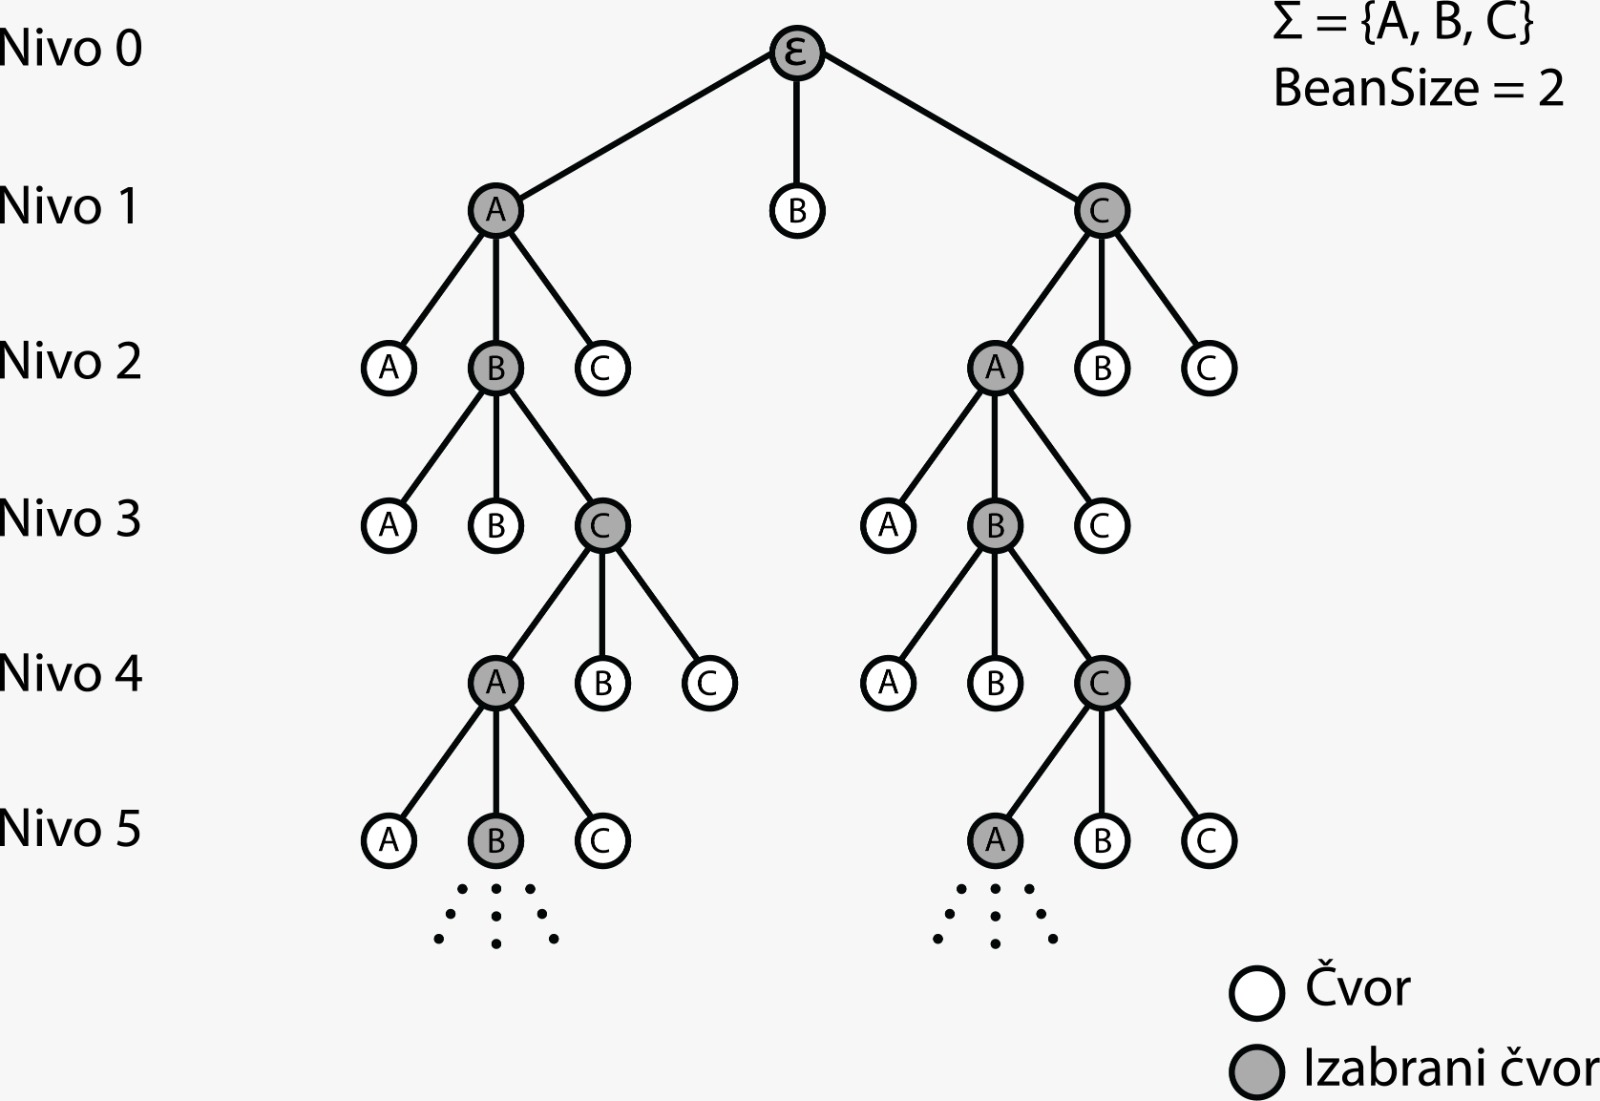
\includegraphics[width=1\textwidth]{Slike/bs1.png}
  \caption{Šema metaheuristike Pretraga Bima} 
  \label{fig:pretragaBima}
\end{figure}
% Sada ćemo predstaviti generalnu ideju Pretrage Bima na kojoj ćemo kasnije izgraditi algoritam za PNZN.
Pretraga Bima predstavlja metaheuristiku koja je uvedena 1976. godine u oblasti prepoznavanja govora
(\textit{eng.} speech recognition). Korišćena je u završnim slojevima mnogih modela za
obradu prirodnog jezika (\textit{eng.} natural language processing models) u donošenju odluke da se izabere najbolji
izlaz date ciljne promenjive \cite{BSIntroduction}. Pored navedenih primena pretraga bima se intenzivno koristi u sledećeim
oblastima: kombinatorna optimizacija (\textit{eng.} combinatorial optimization), problemi planiranja (\textit{eng.} scheduling problems),
problemi rutiranja vozila (\textit{eng.} vehicle routing problems), podešavanje hiperparametara u oblasti mašinskog učenja
(\textit{eng.} Machine Learning Hyperparameter Tuning), problemi zadovoljenja ograničenja (\textit{eng.} Constraint Satisfaction Problems). 

Pretraga Bima predstavlja vrstu pretrage grafa u širinu u cilju da
se pronađe najbolji put od korenog čvora do ciljanog čvora u grafu. Kako bi se složenost izračunavanja držala u
zadatim granicama, Pretraga Bima evaluira dostignute čvorove na određenom nivou ali bira samo podskup od $\beta$
čvorova koji najviše obećavaju i sa tim podskupom čvorova napreduje dalje u pretrazi. Izabrani podskup od $\beta$ čvorova
zvaćemo bim (\textit{eng.} beam) i označavaćemo ga sa $\mathcal{B}$, a $\beta$ parametar ćemo zvati širina bima (\textit{eng.} beam width) \cite{SCSBS}.
U kontekstu PNZN graf koji pretražujemo $\mathcal{G}=(\mathcal{V},\mathbb{E})$ predstavlja usmeren aciklički graf, 
a pseudo kod algoritma je prikazan pod Algoritam \ref{alg:bs}.

Kao i u prethodno opisanom algoritmu podrazumeva se da je promenjiva $maxD$ globalno dostupna,
kao i skupovi $\mathcal{L}$ i $\Sigma$. Svaki element skupa $\mathcal{B}$ predstavlja objekat koji
sadrži parcijalnu reč, heurističku ocenu i pozicije.
Parcijalna reč predstavlja put od korena do nekog čvora unutar stabla pretrage, 
heuristička ocena predstavlja ocenu ove reči od strane heurističke funkcije, a pozicije predstavljaju
niz koji ozančava pozicije do kojih se stiglo unutar skupa $\mathcal{L}$.
Na primer ako je data azbuka $\Sigma=\{a, c, t, g\}$ i skup $\mathcal{L}=\{act,gta,gcc\}$ tada
pozicije $p=[0,0,0]$ predstavljaju baš skup $\mathcal{L}$ odnosno
pozicije na početak svake reči u $\mathcal{L}$, a pozicije $p^{'}=[1,1,2]$ predstavljaju
skup $\mathcal{L}^{'}=\{ct,gt,c\}$ koji je dobijen od skupa $\mathcal{L}$ pomeranjem
za vrednosti pozicija $p^{'}$.  
Pri proširivanju skupa $\mathcal{B}$ slovima iz azbuke $\Sigma$, dobijaju se novi
elementi čija je parcijalna reč proširena novododatim slovom. Od jednog elementa
dobijamo maksimalno $|\Sigma|$ novih, što znači da u svakom koraku algoritma dobijamo
maksimalno $\beta * |\Sigma|$ novih elemenata od kojih je potrebno izabrati $\beta$ 
elemenata. 
Heurističke funkcije, koje će biti predstavljene u narednom podpoglavlju,
za dati niz pozicija računaju težine za svako slovo azbuke, koje se zatim pri proširivanju bima
dodaju svakom elementu koji se proširi odgovarajućim slovom. Ovim se eliminiše potreba za ocenjivanjem
svakog elementa bima iznova i iznova na svakom nivou pretrage, već se heuristička vrednost svakog elementa
inkrementalno gradi. Ovaj vid optimizacije omogućen je samo u slučaju pohlepnih heurističkih funkcija
koje u svakom koraku algoritma u odnosu na redukovan skup $\mathcal{L}$ ocenjuju
novoizabrano slovo.
Nakon proširivanja parcijalne reči odovarajućim slovom azbuke,
vrši se ažuriranje pozicija na taj način što se inkrementiraju pozicije 
onih reči koje počinju izabranim slovom.

Najpre se vrši inicijalizacioni korak algoritma izvan glavne petlje.
Funkcija $\textbf{H}$ predstavlja heurističku funkciju kojoj se inicijalno prosleđuju
pozicije na početak reči iz $\mathcal{L}$. Promenjiva težine sadrži slova i odgovarajuće
težine svakog slova dobijene heurističkom ocenom. Zatim se popunjava bim elementima, gde 
svaki element sadrži slovo azbuke, odgovarajuću težinu
i inicijalne pozicije. Nakon toga vrši se redukcija bima 
kao što je prikazano pod Algoritam \ref{alg:redukujbim}. Ako je veličina bima manja od
dozvoljene širine bima $\beta$ vrši se ažuriranje pozicija svakog elementa kao što je prikazano
pod Algoritam \ref{alg:azurirajPozicije} i vrši se provera da li postoji element koji predstavlja
rešenje PNZN na isti način koji je opisan pod Algoritam \ref{alg:zajNad}.
Ako takav element postoji, postavlja se indikator za kraj algoritma, a pronađena
parcijalna reč se čuva kao rešenje. Ažuriranjem pozicija inkrementiraju se pozicije koje odgovaraj
rečima iz $\mathcal{L}$ počev od trenutnih pozicija, a koje počinju poslednje dodatim slovom.
U slučaju da je veličina bima veća od dozvoljene širine elementi bima se najpre promešaju, a zatim
sortiraju u odnosu na heurističku ocenu. Mešanjem elemenata se eliminiše konstantni azbučni 
poredak kada neki elementi imaju jednaku heurističku vrednost, a time i odabir 
takvih elemenata u azbučnom poretku. Zatim se vrši odabir $\beta$ elemenata sa najvećom 
heurističkom ocenom, pritom se vrši ažuriranje pozicija odabranih elemenata i već opisana
provera zadovoljenja rešenja PNZN. Glavna petlja algoritma prolazi kroz elemente bima, 
i za svaki element se računaju heurističke ocene slova azbuke u odnosu na trenutne pozicije
tog elementa u $\mathcal{L}$. Od svakog elementa dobija se $|\Sigma|$ novih elemenata
proširivanjem parcijalne reči elementa slovima azbuke. Na heurističku vrednost novog elementa
dodaje se heuristička ocena odgovarajućeg slova. Novi element zadržava iste pozicije,
koje se ažuriraju pri redukciji bima ali samo za odabrane elemente, čime se 
izbegava nepotrebno ažuriranje pozicija elemenata koji neće biti izabrani.
Novi elementi se dodaju u bim, nakon čega se vrši redukcija bima na prethodno
opisan način. Algoritam se završava kada pronađe jedno rešenje ili
ako dubina dostigne $maxD$ jer u tom slučaju kao što je već pokazano postoji
jedno trivijalno rešenje problema.
% S obzirom da heuristička funkcija $\textbf{H}$ vraća sortirane težine
% slova, ako u bilo kojoj iteraciji glavne petlje težina prvog slova u sortiranom poretku
% ima vrednost 0, to znači da su pozicije trenutnog elementa    
\\
\begin{algorithm}
  \caption{\textbf{PretragaBimaPNZN()}}
  \label{alg:bs}
  \begin{algorithmic}[1]
  % \Require $n \geq 0$
  % \Ensure $y = x^n$
  \State $b1 \gets \{ \}$
  \State $b2 \gets \{ \}$
  \State $prona\textrm{đ}enaNadniska \gets Neta\textrm{č}no$
  \State
  \State $te\textrm{ž}ine \gets \textbf{H}\textrm{([0,...,0])}$
  \State
  \For{$\alpha\in\Sigma$}
    \State $te\textrm{ž}inaSlova \gets 0$
    \For{$t\in te\textrm{ž}ine$}
      \If{$\alpha == t\textrm{.}slovo$}
        \State $te\textrm{ž}inaSlova \gets t\textrm{.}vrednost$
      \EndIf
    \EndFor
    \State $element \gets \{\alpha\textrm{, }te\textrm{ž}inaSlova \textrm{, [0,...,0]}\}$
    \State $b1\textrm{.}dodaj(element)$
  \EndFor
  \State
  \State $b1 \gets \textbf{RedukujBim}(b1\textrm{, }prona\textrm{đ}enaNadniska)$
  \State $dubina \gets 0$
  \State
  \While{$\neg prona\textrm{đ}enaNadniska \land dubina < maxD$} 
    \For{$s\in b1$}
      \State $te\textrm{ž}ine \gets \textbf{H}(s.pozicije)$
      % \State
      % \If{$te\textrm{ž}ine[0].vrednost == 0$}
      %   \State $\textbf{SkiniPreostalaSlova}()$
      %   \State $prona\textrm{đ}enaNadniska \gets Ta\textrm{č}no$
      %   \State \textbf{break}
      % \EndIf
      \For{$\alpha\in\Sigma$}
        \State $te\textrm{ž}inaSlova \gets 0$
        \For{$t\in te\textrm{ž}ine$}
          \If{$\alpha == t.slovo$}
            \State $te\textrm{ž}inaSlova \gets t.vrednost$
          \EndIf
        \EndFor
      \State $element \gets \{(s.re\textrm{č})\alpha\textrm{, }s.hvrednost + te\textrm{ž}inaSlova\textrm{, }s.pozicije\}$
      \State $b2\textrm{.}dodaj(element)$
      \EndFor
    \EndFor
    \State
    \State $b1\textrm{.}obri\textrm{š}i()$
    \State $b1 \gets \textbf{RedukujBim}(b2\textrm{, }prona\textrm{đ}enaNadniska)$
    \State $b2\textrm{.}obri\textrm{š}i()$
    \State $dubina \gets dubina + 1$
  \EndWhile
  \end{algorithmic}
  \end{algorithm}
\\
\\
\\
\begin{algorithm}
  \caption{$\textbf{RedukujBim}\bm{(\mathcal{B}\textbf{, }prona\textbf{đ}enaNadniska)}$}
  \label{alg:redukujbim}
  \begin{algorithmic}[1]
    \If{$\mathcal{B}.veli\textrm{č}ina() \leqslant \beta$}
      \For{$e \in \mathcal{B}$}
        \State $\textbf{A\textrm{ž}urirajPozicije}(e)$
          \If{$\textbf{ZajedničkaNadniska}(e.re\textrm{č})$}
            \State $nn \gets s.re\textrm{č}$ \Comment{$nn$ - najbolja nadniska}
            \State $nd \gets |nn|$ \Comment{$nd$ - najbolja dužina}
            \State $prona\textrm{đ}enaNadniska \gets Ta\textrm{č}no$
          \EndIf
      \EndFor
      \State \Return $\mathcal{B}$
    \EndIf
    \State
    \State $\textbf{Promešaj}(\mathcal{B})$
    \State $\textbf{Sortiraj}(\mathcal{B})$
    \State $\mathcal{B}\textbf{p} \gets \{ \}$
    \State
    \For{$i=0 \to \beta$}
      \State $\textbf{A\textrm{ž}urirajPozicije}(\mathcal{B}[i])$
      \If{$\textbf{ZajedničkaNadniska}(\mathcal{B}[i].re\textrm{č})}$
            \State $nn \gets \mathcal{B}[i].re\textrm{č}$
            \State $nd \gets |nn|$ 
            \State $prona\textrm{đ}enaNadniska \gets Ta\textrm{č}no$
      \EndIf
      \State $\mathcal{B}\textbf{p}\textrm{.}dodaj(\mathcal{B}[i])$
    \EndFor
    \State
    \State $\mathcal{B}.obri\textrm{š}i()$
    \State \Return $\mathcal{B}\textbf{p}$
  \end{algorithmic}
  \end{algorithm}
\\
Iako algoritam pretrage bima ne garantuje pronalaženje optimalnog rešenja, ovako konstruisan algoritam
ima polinomijalno vreme izvršavanja $O(\beta*maxD)$ što ga u praksi čini daleko efikasnijim od
prethodno opisanog algoritma granja sa odsecanjem. Iz tog razloga će ovaj algoritam biti testiran na
većim instancama PNZN, gde je algoritam grananja sa odsecanjem praktično neizvodljivo testirati
zbog eksponencijalne složenosti.
\\
\begin{algorithm}
  \caption{$\textbf{AžurirajPozicije}\bm{(element)}$}
  \label{alg:azurirajPozicije}
  \begin{algorithmic}[1]
    \State $poslednjeDodatoSlovo \gets element.re\textrm{č}[element.re\textrm{č}.du\textrm{ž}ina() - 1]$
    \State
    \For{$i=0 \to \mathcal{L}.veli\textrm{č}ina()$}
      \If{$\mathcal{L}[i][element.pozicije[i]] == poslednjeDodatoSlovo$}
            \State $element.pozicije[i] \gets element.pozicije[i] + 1$
      \EndIf
    \EndFor
  \end{algorithmic}
  \end{algorithm}
\\
% Algoritam prima tri ulazna parametra: azbuku $\Sigma$, ulazni skup reči $\mathcal{L}$ i širinu bima $\beta$.
% Na početku bim $\mathcal{B}$ predstavlja prazan skup. U svakom koraku algoritma bim se proširuje slovima iz azbuke,
% a zatim se elementi proširenog bima ocenjuje izabranom heurističkom funkcijom. Zatim se vrši odabir $\beta$ čvorova
% sa kojima se dalje nastavlja pretraga, i vrši se provera da li neki čvor u bimu predstavlja rešenje problema,
% ako takav čvor postoji algoritam vraća pronađeno rešenje. Funkcija ProširiBim u prvom koraku popunjava bim slovima
% iz azbuke, a u svakom narednom koraku svako parcijalno rešenje redukovanog bima proširuje dodavajući na njega redom
% slova iz azbuke. Funkcija OceniBim predstavlja heurističku funkciju koja dodeljuje određene vrednosti svakom elementu bima,
% a na osnovu ovih vrednosti funkcija RedukujBim bira $\beta$ parcijalnih rešenja koja imaju najveće vrednosti
% heurističke funkcije. Tokom redukcije bima vrednosti ocena parcijalnih rešenja mogu da se sortiraju tako da redukovani
% bim sadrži $\beta$ najbolje ocenjenih rešenja, ali mogu se koristiti i druge strategije odabira rešenja poput ruletske
% selekcije (\textit{eng.} roulette selection). Funkcija ZajedničkaNadniska vrši proveru da li reč $\omega$
% predstavlja zajedničku nadnisku reči iz skupa $\mathcal{L}$ i jedna njena implementacija će biti opisana u sledećem poglavlju.
% Algoritam se može zaustaviti kada se pronađe prvo rešenje problema, ali mogu se postaviti i drugi uslovi zaustavljanja
% poput broja iteracija petlje (predstavlja dubinu unutar stabla pretrage) ili vremenska ograničenja.

\subsection{Heurističke funkcije Većinsko Spajanje i Težinsko Većinsko Spajanje}
\label{sec:mmiwmm}
Većinsko Spajanje predstavlja jedan od najpopularnijih algoritama koji rešava PNZN. To je pohlepni algoritam
koji inkrementalno konstruiše nadnisku. Najpre se odredi slovo koje se najčešće nalazi na početku reči
iz skupa $\mathcal{L}$, a zatim se izabrano slovo briše sa početka reči iz $\mathcal{L}$ koje ga sadrže.
Postupak se ponavlja dok skup $\mathcal{L}$ ne postane prazan, a dobijena nadniska
predstavlja rešenje PNZN \cite{ProbabilisticBS}.
U kontekstu opisanog algoritma pretrage bima, većinsko spajanje je koršćeno kao heuristička funkcija
koja za dati niz pozicija u $\mathcal{L}$ vraća objekat koji sadrži slova azbuke i odgovarajuće
težine u udnosu na to koliko reči od odgovarajućih pozicija počinje odgovarajućim slovom.
Nakon izračunavanja težina, vrši se mešanje i sortiranje vrednosti. Mešanje nije neophodno,
ali kao što je već rečeno eliminiše se konstantan azbučni poredak. 

\begin{algorithm}
  \caption{\textbf{VećinskoSpajanje(pozicije)}}
  \label{alg:mm}
  \begin{algorithmic}[1]
  % \Require $n \geq 0$
  % \Ensure $y = x^n$
  \State $te\textrm{ž}ine \gets \{\alpha \in \Sigma\textrm{, }[0,...,0] \}$ \Comment{inicijalizacija težina}
  \State
  \For{$i=0 \to \mathcal{L}.veli\textrm{č}ina()$}
    \If{$pozicije[i] \leq (\mathcal{L}[i].du\textrm{ž}ina() - 1)$}
      \For{$t \in te\textrm{ž}ine$}
        \If{$t.slovo == \mathcal{L}[i][pozicije[i]]$}
          \State $t.vrednost \gets t.vrednost + 1$
        \EndIf 
      \EndFor
    \EndIf 
  \EndFor
  \State
  \State $\textbf{Promešaj}(te\textrm{ž}ine)$
  \State $\textbf{Sortiraj}(te\textrm{ž}ine)$
  \State
  \State \Return $te\textrm{ž}ine$
  \end{algorithmic}
  \end{algorithm}

Pseudo kod algoritma prikazan je pod Algoritam \ref{alg:mm}.
Mana Većinskog Spajanja je to što ne može da prepozna globalnu strukturu reči iz skupa $\mathcal{L}$.
U principu Većinsko spajanje izostavlja činjenicu da reči mogu biti različitih dužina. To dalje 
znači da će slova sa početka kraćih reči imati veću šansu da budu uklonjena iako algoritam i dalje treba
da obradi preostale dugačke reči. Iz tog razloga bi skidanje slova sa početka kraćih reči trebalo da bude
manje prioritetno. Drugim rečima bolje je da se prioritizira skidanje slova sa početka dužih reči.
To se može postići dodavanjem težine svakom slovu azbuke u odnosu na dužinu preostalih reči iz $\mathcal{L}$ 
nakon uklanjanja tog simbola sa početka reči koje počinju tim simbolom. Dakle korak 7 u algoritmu VećinskoSpajanje
možemo zameniti sa:
\\
\\
\begin{equation}
  \label{eqn:wmm}
  t.vrednost \gets t.vrednost + (\mathcal{L}[i].du\textrm{ž}ina() - 1) - pozicije[i]
\end{equation}
\\
\\
Ovako modifikovan algoritam naziva se Težinsko Većinsko Spajanje i postoje indikacije da na određenim instancama
problema može da nadmaši algoritam Većinskog Spajana, pogotovo kada nema struktuiranosti unutar skupa $\mathcal{L}$
ili kada je ta struktuiranost haotična \cite{ProbabilisticBS}. Predstavljene dve heurističke
funkcije su korišćene u algoritmu pretrage bima.

\chapter{Evaluacija algoritama}
\label{chap:evaluacijaAlg}
U ovom poglavlju biće prikazani rezultati izvršavanja predstavljenih algoritama
kao i test podaci koji su korišćeni za testiranje i način na koji su test podaci generisani.
Takođe će biti dat kratak pregled eksperimentalnog okruženja u kome se vršilo testiranje,
hardverska i softverska specifikacija računara kao i specifičnosti implementacije.

\section{Test podaci}
\label{sec:testPodaci}
Za uspešno testiranje rada predstavljenih algoritama pored instanci problema najkraće
zajedničke nadniske
$IP = \{\mathcal{I}_{1}(\Sigma_{1},\mathcal{L}_{1}),...,\mathcal{I}_{k}(\Sigma_{k},\mathcal{L}_{k})\}$
neophodno je da postoji barem jedno optimalno rešenje $\mathcal{R}_{i}$ za svaku
instancu problema $\mathcal{I}_{i}$. Takvo rešenje najčešće nije jedinstveno,
a broj optimalnih rešenja varira od instance do instance problema i raste sa porastom
broja reči u skupu $\mathcal{L}$. Ono što je bitno, jeste dužina takvog rešenja i to je
jedini validan parametar optimalnosti. Algoritam pretrage bima ne garantuje pronalaženje
optimalnog rešenja dok algoritam grananja sa odsecanjem garantuje. Naizgled on može poslužiti
za testiranje algoritma pretrage bima, ali
vreme izvšavanja grananja sa odsecanjem eksponencijalno raste sa porastom parametra $maxD$
pa vreme izvšavanja ovog algoritma čak i na manjim instancama PNZN postaje predugo.
Na primer ako najduža reč u skupu $\mathcal{L}$ ima dvadeset slova i pritom je
data proizvoljna azbuka kardinalnosti $|\Sigma|=4$, u najgorem slučaju
algoritam grananja sa odsecanjem treba da obradi $(4^{80}-1)/3$ čvorova.
S obzirom na navedene činjenice i manjak test podataka u literaturi, osmišljen je
algoritam koji generiše test instance. Pseudo kod algoritma je prikazan pod
Algoritam \ref{alg:generatorTestInstanci}. Ideja je da se odabere reč koja će 
predstavljati gornju granicu optimalnosti i da se na osnovu odabrane reči
generišu instance problema.
Generator test instanci ima četiri parametra: $putanja$ predstavlja putanju do
tekstualnog fajla koji sadrži reč koja predstavlja gornju granicu, $n$ označava
broj slova u azbuci $\Sigma$, $m$ označava broj reči u skupu $\mathcal{L}$,
a parametar $\gamma$ predstavlja verovatnoću uklanjanja slova iz $gg$ pri generisanju
reči. Najpre se učitava reč $gg$ sa odabrane lokacije i azbuka popunjava
odabranim slovima. Zatim se popunjava skup $\mathcal{L}$.
U svakoj iteraciji petlje se kreće od prazne reči $\omega$, prolazi se
kroz slova $gg$ i bira se slučajan broj iz uniformne raspodele (u granicama [0,1]).
Ako je odabrani slučajan broj veći od $\gamma$, reč $\omega$ se proširuje
trenutnim slovom. Zapravo, reč $\omega$ predstavlja reč koja se dobija uklanjanjem slova iz 
reči $gg$ sa verovatnoćom $\gamma$.
Na ovaj način se generiše $m$ reči kojima se popunjava skup $\mathcal{L}$, a algoritam
na kraju vraća jednu generisanu instancu problema $\mathcal{I}(\Sigma,\mathcal{L})$.
\\
\begin{algorithm}
  \caption{\textbf{GeneratorTestInstanci}\bm{$(putanja,n,m,\gamma)$}}
  \label{alg:generatorTestInstanci}
  \begin{algorithmic}[1]
  \State $gg \gets \textbf{Pročitaj}(putanja)$ \Comment{$gg$ - gornja granica}
  \State $\Sigma \gets \{\}$
  \State $\mathcal{L} \gets \{\}$
  \State

  \For{$i \to n$} 
    \State $\alpha \gets \textbf{PročitajSlovo}()$
    \State $\Sigma .dodaj(\alpha)$
  \EndFor
  \State
  \For{$i \to m$} 
    \State $\omega \gets \varepsilon$
    \For{$s \in gg$}
      \State $slu\textrm{č}ajanBroj \gets \textbf{GenerišiSlučajanBroj}()$
      \If{$slu\textrm{č}ajanBroj > \gamma$}
        \State $\omega .dodaj(s)$
      \EndIf
    \EndFor
    \State
    \State $\mathcal{L} .dodaj(\omega)$
    \State
  \EndFor
  \State
  \State $\mathcal{I} \gets (\Sigma,\mathcal{L})$
  \State
  \State \Return $\mathcal{I}$
  \end{algorithmic}
  \end{algorithm}
\\
Preostalo je još objasniti na koji način se generiše reč koja predstavlja gornju granicu.
Reč $gg$ dobija se slučajnim odabirom slova iz azbuke. U svakoj iteraciji 
izgradnje bira se slučajan broj $sb$ iz uniformne
raspodele (u granicama [0,$|\Sigma|-1$]) i parcijalnoj reči dodaje 
odgovarajuće slovo azbuke $\Sigma[sb]$.
Gornja granica optimalnosti garantuje jedno rešenje problema. Uz pažljivo odabran parametar
$\gamma$ i dovoljno veliki parametar $m$ gornja granica će skoro uvek i predstavljati
optimalno rešenje problema. U svakom slučaju gornja granica će u kontekstu testiranja
predstavljenih algoritama biti sinonim za optimalno rešenje i poređenje rezultata će se
vršiti u odnosu na njenu dužinu.

Sada će biti definisan skup instanci problema $IP$ koji je korišćen za testiranje u sekciji \ref{sec:ekspRezultati}.
Postoje četiri bitna parametra koja su korišćena za generisanje instanci PNZN:
\begin{enumerate}
  \item Veličina azbuke $\Sigma$ ($n=|\Sigma|$)
  \item Broj reči u skupu $\mathcal{L}$ ($m=|\mathcal{L}|$)
  \item Dužina gornje granice ($|gg|$)
  \item Verovatnoća uklanjanja slova ($\gamma$)
\end{enumerate}
Veličina azbuke uzeta je iz opsega $n \in \{2,4,16 \}$, broj reči u skupu $\mathcal{L}$
iz opsega $m \in \{10,20,40,80\}$. Dužina gornje granice definiše i potencijalnu gornju
granicu za dužinu reči u skupu $\mathcal{L}$ i ona je uzeta iz opsega $|gg| \in \{50,100,500,2000\}$.
Na kraju verovatnoća uklanjanja slova uzeta je iz opsega $\gamma \in \{0.1,0.2,0.4\}$.
Instance problema podeljene su u tri skupa $IP_{\gamma=0.1}$, $IP_{\gamma=0.2}$ i $IP_{\gamma=0.4}$
na osnovu verovatnoće uklanjanja slova. Sva tri skupa sadrže po 48 instanci problema
koje su dobijene kao dekartov proizvod vrednosti prethodno opisanih parametara.
Vrednosti za širinu bima uzete su iz opsega $\beta \in \{100,200,400\}$.
Algoritam grananja sa odsecanjem testiran je na manjem skupu instanci
$IPG$ gde $n \in \{2,4\}$, $m \in \{8,16,32\}$. Gornja granica za azbuku dužine dva
uzeta je iz opsega $|gg|_{|\Sigma|=2} \in \{20,24,28\}$, a za azbuku dužine četiri
$|gg|_{|\Sigma|=4} \in \{12,13,14\}$ kako bi se vreme izvršavanja držalo u razumnim
granicama. Instance problema podeljene su u dva skupa $IPG_{\gamma=0.2}$ i $IPG_{\gamma=0.4}$
na osnovu verovatnoće uklanjanja slova i svaki skup sadrži po 18 instanci problema.
% $IPG$, sa verovatnoćom uklanjanja $\gamma=0.2$, $n \in \{2,4\}$, $m \in \{8,16,32\}$
% i $|gg| \in \{20,24,28\}$.

\section{Eksperimentalno okruženje}
\label{sec:ekspOkruženje}
U ovoj sekciji će biti dat kratak pregled hardverske i softverske konfiguracije
računara na kome se vršilo testiranje kao i specifičnosti implementacije
predstavljenih algoritama.
\subsection{Hardversko i softversko okruženje}
\label{sec:hardSoft}
Svi rezultati izvršavanja algoritama dobijeni su na računaru pod Linux operativnim sistemom
sledećih sistemskih specifikacija:
\begin{itemize}
  \item Operativni sistem - Ubuntu 20.04.6 LTS
  \item Kernel - Linux 5.15.0-46-generic
  % \item Arhitektura - x86-64
\end{itemize}
Hardverske komponente računara na kome se vršilo testiranje su sledeće:
\begin{itemize}
  \item Procesor - AMD Ryzen 3 1300X, 3.5GHz
  \item Arhitektura - x86-64
  \item Broj jezgara - 4
  \item Keš memorija - L1(384KiB), L2(2MiB), L3(8MiB)
  \item Ram memorija - Kingston, 8GB DDR4
  \item Grafička kartica - Asus Radeon RX 570 (4GB GDDR5)
\end{itemize}
Treba napomenuti još to da iako procesor ima četiri jezgra i četiri
fizičke niti, algoritmi nisu implementirani tako da podržavaju paralelno izvršavanje.

\subsection{Specifičnosti implementacije i pokretanje programa}
\label{sec:specifinicnostiImplementacije}
Svi predstavljeni algoritmi u radu implementirani su u programskom jeziku C++
kako bi se postigla što veća efikasnost u evaluaciji. Korišćen je
GCC 9.4.0 prevodilac i standard jezika C++20. Ceo programski kod je organizovan
unutar klase, a svi prethodno navedeni algoritmi i pomoćne funkcije kao privatne
funckije članice (\textit{eng.} member function) kako bi podrazumevano bile
utisnute (\textit{eng.} inline) na mestima u programu na kojima se pozivaju i kako
bi se time izbegli nepotrebni troškovi poziva. U cilju što veće optimizacije
određenih delova programskog koda, iako u današnje vreme ne popularne,
korišćene su i pokazivačke promenjive i odgovarajuća aritmetika. 
Implementacija svih struktura podataka poput skupova, vektora, uređenih parova
uzeta je iz standardne biblioteke C++ jezika (\textit{eng.} Standard C++ Library), kao i svi
pomoćni algoritmi poput sortiranja ili mešanja elemenata.
Svi generatori slučajnih brojeva koji su korišćeni sadrže fiksiranu
vrednost semena (\textit{eng.} seed), kako bi generisanje test instanci
i evaluacija algoritama mogla da se reprodukuje u definisanim uslovima.
Sve generisane test instance i odgovarajući rezultati nalaze se u numerisanim tekstualnim fajlovima.
Programski kod je organizovan u dva cpp fajla i prevodi se korišćenjem
pomoćnog alata Make. Prilikom prevođenja upaljen je najviši nivo
optimizacije od strane GCC prevodioca postavljanjem parametra -O3.
Prevođenje i pokretanje odgovarajućih programa vrši se
iz Linux terminala na sledeći način:
\begin{itemize}
  \item make testInstanceGenerator - prevodi generator test instanci
  \item make SCS - prevodi program koji pokreće opisane algoritme
  \item ./testInstanceGenerator (režim rada) - pokreće generator test instanci koji nakon poziva 
  očekuje putanju do tekstualnog fajla u kome se nalazi reč koja predstavlja gornju granicu,
  broj reči m, i željena slova azbuke (parametar $\gamma$ se postavlja u kodu pre prevođenja),
  izlaz je numerisan tekstualni fajl koji predstavlja jednu instancu PNZN (postoji više 
  režima rada generatora, na primer prethodno opisani podrazumeva ulazni argument 2, dok je za generisanje
  reči $gg$ potrebno navesti ulazni argument 3)
  \item ./SCS (broj test instance) - pokreće program koji izvršava algoritme,
  kao ulazni argument očekuje redni broj test instance, izlaz je numerisan tekstualni fajl
  koji sadrži rezultat izvršavanja ulazne test instance
\end{itemize}
% Pre prikaza eksperimentalnih rezultata izvršavanja algoritama,
% potrebno je još prodiskutovati širinu bima, odnosno metaparametar $\beta$.
% Vrednosti širine bima uzete su iz opsega $\beta \in \{100,200,400\}$.

\section{Eksperimentalni rezultati}
\label{sec:ekspRezultati}
U ovoj sekciji biće prikazani eksperimentalni rezultati izvršavanja algoritama.
U tabeli \ref{tbl:gso} prikazani su rezultati algoritma grananja sa odsecanjem,
na skupu test instanci $IPG_{\gamma=0.2}$ i $IPG_{\gamma=0.4}$. 
Kolone redom označavaju: veličinu ulazne azbuke $\Sigma$ ($n=|\Sigma|$),
broj reči u skupu $\mathcal{L}$ ($m=|\mathcal{L}|$), dužinu gornje granice ($|gg|$),
dužinu nadniske koju je algoritam granja sa odsecanjem pronasao ($GSO$),
vreme izvršavanja algoritma ($t$),
minimalnu dubinu pretrage ($minD$),
maksimalnu dubinu pretrage ($maxD$).
U tabelama \ref{tbl:bs1}, \ref{tbl:bs2}, \ref{tbl:bs3} predstavljeni su rezultati
izvršavanja algoritma pretrage bima na test instancama
$IP_{\gamma=0.1}$, $IP_{\gamma=0.2}$, $IP_{\gamma=0.4}$.
% \begin{enumerate}
%   \item Veličinu ulazne azbuke $\Sigma$ ($n=|\Sigma|$)
%   \item Broj reči u skupu $\mathcal{L}$ ($m=|\mathcal{L}|$)
%   \item Dužinu gornje granice ($|gg|$)
%   \item Dužinu nadniske koju je algoritam granja sa odsecanjem pronasao ($GSO$)
%   \item Vreme izvršavanja algoritma ($t$)
%   \item Minimalnu dubinu pretrage (minD)
%   \item Maksimalnu dubinu pretrage (maxD)
% \end{enumerate}

\begin{table}[H]
\centering
\begin{tabular}{ |P{0.5cm}|P{0.5cm}|P{0.5cm}||P{1cm}|P{0.7cm}|P{1cm}|P{1cm}| }
  \hline
  \multicolumn{7}{|c|}{$IPG_{\gamma=0.2}$} \\
  \hline
  $|\Sigma|$ & $m$ & $|gg|$ & $GSO$ & $t(s)$ & $minD$ & $maxD$\\
  \hline
  2  & 8 & 20 & 20 & 1 & 19 & 38\\
  \hline
  2 & 8 & 24 & 24 & 6 & 21 & 42\\
  \hline
  2 & 8 & 28 & 28 & 101 & 24 & 48\\
  \hline
  2 & 16 & 20 & 20 & 0 & 19 & 38\\
  \hline
  2 & 16 & 24 & 24 & 6 & 21 & 42\\
  \hline
  2 & 16 & 28 & 28 & 105 & 26 & 52\\
  \hline
  2 & 32 & 20 & 20 & 0 & 19 & 38\\
  \hline
  2 & 32 & 24 & 24 & 6 & 22 & 44\\
  \hline
  2 & 32 & 28 & 28 & 108 & 26 & 52\\
  \hline
  4  & 8 & 12 & 12 & 4 & 11 & 44\\
  \hline
  4  & 8 & 13 & 13 & 15 & 13 & 52\\
  \hline
  4  & 8 & 14 & 14 & 64 & 14 & 56\\
  \hline
  4  & 16 & 12 & 12 & 4 & 11 & 44\\
  \hline
  4  & 16 & 13 & 13 & 15 & 13 & 52\\
  \hline
  4  & 16 & 14 & 14 & 63 & 14 & 56\\
  \hline
  4  & 32 & 12 & 12 & 4 & 12 & 48\\
  \hline
  4  & 32 & 13 & 13 & 15 & 13 & 52\\
  \hline
  4  & 32 & 14 & 14 & 64 & 14 & 56\\
  \hline
  \multicolumn{7}{|c|}{$IPG_{\gamma=0.4}$} \\
  \hline
  2  & 8 & 20 & 18 & 0 & 14 & 28\\
  \hline
  2  & 8 & 24 & 21 & 1 & 16 & 32\\
  \hline
  2  & 8 & 28 & 25 & 8 & 18 & 36\\
  \hline
  2  & 16 & 20 & 19 & 0 & 14 & 28\\
  \hline
  2  & 16 & 24 & 21 & 1 & 16 & 32\\
  \hline
  2  & 16 & 28 & 26 & 27 & 21 & 42\\
  \hline
  2  & 32 & 20 & 20 & 0 & 16 & 32\\
  \hline
  2  & 32 & 24 & 23 & 4 & 20 & 40\\
  \hline
  2  & 32 & 28 & 27 & 53 & 23 & 46\\
  \hline
  4  & 8 & 12 & 12 & 3 & 9 & 36\\
  \hline
  4  & 8 & 13 & 13 & 17 & 11 & 44\\
  \hline
  4  & 8 & 14 & 14 & 60 & 10 & 40\\
  \hline
  4  & 16 & 12 & 12 & 4 & 9 & 36\\
  \hline
  4  & 16 & 13 & 13 & 16 & 11 & 44\\
  \hline
  4  & 16 & 14 & 14 & 60 & 10 & 40\\
  \hline
  4  & 32 & 12 & 12 & 4 & 9 & 36\\
  \hline
  4  & 32 & 13 & 13 & 17 & 11 & 44\\
  \hline
  4  & 32 & 14 & 14 & 65 & 11 & 44\\
  \hline
 \end{tabular}
 \caption{Rezultati grananja sa odsecanjem na test instancama $IPG_{\gamma=0.2}$ i  $IPG_{\gamma=0.4}$}
 \label{tbl:gso}
\end{table}


\begin{table}[H]
  \centering
  \scalebox{0.8}{
  \begin{tabular}{ |P{0.5cm}|P{0.5cm}|P{0.7cm}||P{0.7cm}|P{0.5cm}|P{0.8cm}|P{0.5cm}| P{0.7cm}|P{0.5cm}|P{0.8cm}|P{0.5cm}| P{0.7cm}|P{0.5cm}|P{0.8cm}|P{0.5cm}|}
    \hline
    \multicolumn{15}{|c|}{$IP_{\gamma=0.1}$} \\
    \hline
    \multicolumn{3}{|c||}{}  & \multicolumn{4}{c|}{$\beta=100$} & \multicolumn{4}{c|}{$\beta=200$} & \multicolumn{4}{c|}{$\beta=400$}\\
    \hline
    $|\Sigma|$ & $m$ & $|gg|$ & $VS$ & $t(s)$ & $TVS$ & $t(s)$ & $VS$ & $t(s)$ & $TVS$ & $t(s)$ & $VS$ & $t(s)$ & $TVS$ & $t(s)$\\
    \hline
    2 &	10 & 50 &	50 & 0 & 50 &	0 & 50 & 0 & 50 & 0 & 50 & 0 & 50 & 0\\
    \hline
    2	& 10 & 100 & 100 & 0 & 100 & 0 & 100 & 0 & 100 & 0 & 100 & 0 & 100 & 0\\
    \hline
    2	& 10 & 500 & 500 & 0 & 500 & 0 & 500 & 0 & 500 & 0 & 500 & 0 & 500 & 0\\
    \hline
    2 & 10 & 2000 & 2000 & 1 & 2000 & 0 & 2000 & 1 & 2000 & 1 & 2000 & 3 & 2000 & 2\\
    \hline
    2	& 20 & 50 & 50 & 0 & 50 & 0 & 50 & 0 & 50 & 0 & 50 & 0 & 50 & 0\\
    \hline
    2	& 20 & 100 & 100 & 0 & 100 & 0 & 100 & 0 & 100 & 0 & 100 & 0 & 100 & 0\\
    \hline
    2	&20&	500&		500&	0&	500&	0&	500&	0&	500&	0&	500&	1&	500&	0\\
    \hline
    2	&20	&2000	&	2000	&1 & 2000 &	0&	2000&	2&	2000&	1&	2000&	3&	2000&	3\\
    \hline
    2	&40&	50&		50&	0&	50&	0&	50&	0&	50&	0&	50&	0&	50&	0\\
    \hline
    2	&40&	100&		100&	0&	100&	0&	100&	0&	100&	0&	100&	0&	100&	0\\
    \hline
    2	&40&	500&		500&	0&	500&	0&	500&	1&	500&	0&	500&	0&	500&	1\\
    \hline
    2	&40&	2000&		2000&	1&	2000&	1&	2000&	2&	2000&	1&	2000&	4&	2000&	3\\
    \hline
    2	&80&	50&		50&	0&	50&	0&	50&	0&	50&	0&	50&	0&	50&	0\\
    \hline
    2&	80&	100&	100&	0&	100&	0&	100&	0&	100&	0&	100&	0&	100&	0\\
    \hline
    2&	80&	500&	500&	1&	500&	0&	500&	1&	500&	0&	500&	1&	500&	0\\
    \hline
    2&	80&	2000&		2000&	1&	2000&	1&	2000&	2&	2000&	3&	2000&	5&	2000&	5\\
    \hline
    4 &	10&	50&	50&	0&	50&	0&	50&	0&	50&	0&	50&	0&	50&	0\\
    \hline
    4 & 10&	100 & 100&	0&	100&	0&	100&	0&	100&	0&	100&	0&	100&	0\\
    \hline
    4&	10&	500& 500&	0&	500&	0&	500&	0&	500&	1&	500&	0&	500&	1\\
    \hline
    4&	10&	2000&		2000&	1&	2000&	0&	2000&	2&	2000&	1&	2000&	4&	2000&	3\\
    \hline
    4	& 20&	50&	50&	0&	50&	0&	50&	0&	50&	0&	50&	0&	50&	0\\
    \hline
    4	& 20&	100&	100&	0&	100&	0&	100&	0&	100&	0&	100&	0&	100&	0\\
    \hline
    4	& 20&	500&	500&	0&	500&	0&	500&	0&	500&	0&	500&	1&	500&	0\\
    \hline
    4&	20&	2000&		2000&	1&	2000&	1&	2000&	2&	2000&	2&	2000&	4&	2000&	4\\
    \hline
    4&	40&	50&	50&	0&	50&	0&	50&	0&	50&	0&	50&	0&	50&	0\\
    \hline
    4	& 40&	100&	100&	0&	100&	0&	100&	0&	100&	0&	100&	0&	100&	0\\
    \hline
    4&	40&	500&	500&	0&	500&	0&	500&	1&	500&	0&	500&	1&	500&	0\\
    \hline
    4&	40&	2000&	2000&	2&	2000&	1&	2000&	3&	2000&	2&	2000&	5&	2000&	5\\
    \hline
    4&	80&	50&	50&	0&	50&	0&	50&	0&	50&	0&	50&	0&	50&	0\\
    \hline
    4	& 80&	100&	100&	0&	100&	0&	100&	0&	100&	0&	100&	0&	100&	0\\
    \hline
    4&	80&	500&	500&	0&	500&	0&	500&	1&	500&	0&	500&	1&	500&	1\\
    \hline
    4 &	80&	2000&		2000&	2&	2000&	1&	2000&	3&	2000&	3&	2000&	6&	2000&	7\\
    \hline
    16&	10&	50&	50&	0&	50&	0&	50&	0&	50&	0&	50&	0&	50&	0\\
    \hline
    16&	10&	100&	100&	0	& 100&	0&	100&	0&	100&	0&	100&	1&	100&	0\\
    \hline
    16&	10&	500&	500&	0&	500&	0&	500&	1&	500&	0&	500&	1&	500&	1\\
    \hline
    16&	10&	2000&		2000&	2&	2000&	2&	2000&	5&	2000&	5&	2000&	11&	2000&	11\\
    \hline
    16&	20&	50&		50&	0&	50&	0&	50&	0&	50&	0&	50&	0&	50&	0\\
    \hline
    16&	20&	100&	100&	0&	100&	0&	100&	0&	100&	0&	100&	1&	100&	0\\
    \hline
    16&	20&	500&	500&	0&	500&	0&	500&	1&	500&	0&	500&	1&	500&	1\\
    \hline
    16&	20&	2000&	2000&	2&	2000&	2&	2000&	5&	2000&	5&	2000&	11&	2000&	11\\
    \hline
    16&	40&	50&	50&	0&	50&	0&	50&	0&	50&	0&	50&	0&	50&	0\\
    \hline
    16&	40&	100&	100&	0&	100&	0&	100&	0&	100&	0&	100&	0&	100&	0\\
    \hline
    16&	40&	500&	500&	0&	500&	0&	500&	1&	500&	0&	500&	2&	500&	1\\
    \hline
    16 &	40&	2000&	2000&	3&	2000&	2&	2000&	6&	2000&	5&	2000&	13&	2000&	12\\
    \hline
    16&	80&	50&		50&	0&	50&	0&	50&	0&	50&	0&	50&	0&	50&	0\\
    \hline
    16&	80&	100&	100&	0&	100&	0&	100&	0&	100&	0&	100&	1&	100&	0\\
    \hline
    16 &	80&	500&	500&	0&	500&	0&	500&	1&	500&	1&	500&	2&	500&	2\\
    \hline
    16 &	80&	2000&		2000&	4&	2000&	3&	2000&	7&	2000&	7&	2000&	15&	2000&	15\\
    \hline
   \end{tabular}
  }
   \caption{Rezultati pretrage bima na test instancama $IP_{\gamma=0.1}$}
   \label{tbl:bs1}
  \end{table}

  \begin{table}[H]
    \centering
    \scalebox{0.8}{
    \begin{tabular}{ |P{0.5cm}|P{0.5cm}|P{0.7cm}||P{0.7cm}|P{0.5cm}|P{0.8cm}|P{0.5cm}| P{0.7cm}|P{0.5cm}|P{0.8cm}|P{0.5cm}| P{0.7cm}|P{0.5cm}|P{0.8cm}|P{0.5cm}|}
      \hline
      \multicolumn{15}{|c|}{$IP_{\gamma=0.2}$} \\
      \hline
      \multicolumn{3}{|c||}{}  & \multicolumn{4}{c|}{$\beta=100$} & \multicolumn{4}{c|}{$\beta=200$} & \multicolumn{4}{c|}{$\beta=400$}\\
      \hline
      $|\Sigma|$ & $m$ & $|gg|$ & $VS$ & $t(s)$ & $TVS$ & $t(s)$ & $VS$ & $t(s)$ & $TVS$ & $t(s)$ & $VS$ & $t(s)$ & $TVS$ & $t(s)$\\
      \hline
      2 &	10 & 50	&	50&	0&	50&	0&	50&	0&	50&	0&	50&	0&	50&	0\\
      \hline
      2&	10&	100&	100&	0&	100&	0&	100&	0&	100&	0&	100&	0&	100&	0\\
      \hline
      2&	10&	500&	589&	0&	563&	0&	558&	0&	574&	0&	561&	0&	546&	0\\
      \hline
      2&	10&	2000&	2346&	1&	2320&	1&	2364&	3&	2326&	2&	2311&	4&	2273&	4\\
      \hline
      2&	20&	50&	50&	0&	50&	0&	50&	0&	50&	0&	50&	0&	50&	0\\
      \hline
      2&	20&	100&	100&	0&	100&	0&	100&	0&	100&	0&	100&	0&	100&	0\\
      \hline
      2&	20&	500&	503&	0&	499&	0&	499&	0&	499&	0&	499&	1&	499&	0\\
      \hline
      2&	20&	2000&	2474&	3&	2269&	1&	2380&	2&	2288&	2&	2432&	4&	2310&	4\\
      \hline
      2&	40&	50&	50&	0&	50&	0&	50&	0&	50&	0&	50&	0&	50&	0\\
      \hline
      2&	40&	100&	100&	0&	100&	0&	100&	0&	100&	0&	100&	0&	100&	0\\
      \hline
      2&	40&	500&	500&	0&	500&	0&	620&	1&	610&	1&	500&	1&	500&	0\\
      \hline
      2	&40&	2000&		1999&	3&	1999&	1&	1999&	2&	1999&	2&	1999&	4&	1999&	4\\
      \hline
      2&	80&	50&	50&	0&	50&	0&	50&	0&	50&	0&	50&	0&	50&	0\\
      \hline
      2&	80&	100&	100&	0&	100&	0&	100&	0&	100&	0&	100&	0&	100&	0\\
      \hline
      2&	80&	500&	500&	0&	500&	0&	500&	1&	500&	0&	500&	1&	500&	0\\
      \hline
      2&	80&	2000&	2208&	3&	2200&	3&	2207&	6&	2193&	5&	2000&	5&	2000&	4\\
      \hline
      4&	10&	50&	50&	0&	50&	0&	50&	0&	50&	0&	50&	0&	50&	0\\
      \hline
      4&	10&	100&	100&	0&	100&	0&	100&	0&	100&	0&	100&	0&	100&	0\\
      \hline
      4&	10&	500&	500&	1&	500&	0&	500&	1&	500&	0&	500&	1&	500&	0\\
      \hline
      4&	10&	2000&	2000&	1&	2000&	0&	2000&	2&	2000&	1&	2000&	4&	2000&	4\\
      \hline
      4&	20&	50&	50&	0&	50&	0&	50&	0&	50&	0&	50&	0&	50&	0\\
      \hline
      4&	20&	100&	100&	0&	100&	0&	100&	0&	100&	0&	100&	0&	100&	0\\
      \hline
      4&	20&	500&	500&	0&	500&	0&	500&	0&	500&	0&	500&	1&	500&	0\\
      \hline
      4&	20&	2000&	2000&	1&	2000&	1&	2000&	2&	2000&	2&	2000&	4&	2000&	4\\
      \hline
      4&	40&	50&	50&	0&	50&	0&	50&	0&	50&	0&	50&	0&	50&	0\\
      \hline
      4&	40&	100&	100&	0&	100&	0&	100&	0&	100&	0&	100&	0&	100&	0\\
      \hline
      4&	40&	500&	500&	0&	500&	0&	500&	0&	500&	0&	500&	1&	500&	0\\
      \hline
      4&	40&	2000&	2000&	1&	2000&	1&	2000&	2&	2000&	2&	2000&	5&	2000&	5\\
      \hline
      4&	80&	50&	50&	0&	50&	0&	50&	0&	50&	0&	50&	0&	50&	0\\
      \hline
      4&	80&	100&	100&	0&	100&	0&	100&	0&	100&	0&	100&	0&	100&	0\\
      \hline
      4&	80&	500&	500&	0&	500&	0&	500&	1&	500&	0&	500&	1&	500&	1\\
      \hline
      4&	80&	2000&	2000&	2&	2000&	1&	2000&	3&	2000&	3&	2000&	7&	2000&	7\\
      \hline
      16&	10&	50&	50&	0&	50&	0&	50&	0&	50&	0&	50&	0&	50&	0\\
      \hline
      16&	10&	100&	100&	0&	100&	0&	100&	0&	100&	0&	100&	0&	100&	0\\
      \hline
      16&	10&	500&	500&	1&	500&	0&	500&	1&	500&	1&	500&	1&	500&	1\\
      \hline
      16&	10&	2000&	2000&	2&	2000&	2&	2000&	4&	2000&	5&	2000&	11&	2000&	10\\
      \hline
      16&	20&	50&	50&	0&	50&	0&	50&	0&	50&	0&	50&	0&	50&	0\\
      \hline
      16&	20&	100&	100&	0&	100&	0&	100&	0&	100&	0&	100&	0&	100&	0\\
      \hline
      16&	20&	500&	500&	0&	500&	0&	500&	1&	500&	0&	500&	1&	500&	1\\
      \hline
      16&	20&	2000&	2000&	2&	2000&	2&	2000&	5&	2000&	5&	2000&	11&	2000&	11\\
      \hline
      16&	40&	50&	50&	0&	50&	0&	50&	0&	50&	0&	50&	0&	50&	0\\
      \hline
      16&	40&	100&	100&	0&	100&	0&	100&	0&	100&	0&	100&	0&	100&	0\\
      \hline
      16&	40&	500&	500&	1&	500&	0&	500&	1&	500&	1&	500&	2&	500&	2\\
      \hline
      16&	40&	2000&	2000&	3&	2000&	2&	2000&	6&	2000&	6&	2000&	13&	2000&	13\\
      \hline
      16&	80&	50&	50&	0&	50&	0&	50&	0&	50&	0&	50&	0&	50&	0\\
      \hline
      16&	80&	100&	100&	0&	100&	0&	100&	0&	100&	0&	100&	1&	100&	0\\
      \hline
      16&	80&	500&	500&	1&	500&	0&	500&	1&	500&	1&	500&	2&	500&	2\\
      \hline
      16&	80&	2000&	2000&	3&	2000&	4&	2000&	7&	2000&	7&	2000&	16&	2000&	15\\
      \hline
     \end{tabular}
    }
     \caption{Rezultati pretrage bima na test instancama $IP_{\gamma=0.2}$}
     \label{tbl:bs2}
    \end{table}


    \begin{table}[H]
      \centering
      \scalebox{0.8}{
      \begin{tabular}{ |P{0.5cm}|P{0.5cm}|P{0.7cm}||P{0.7cm}|P{0.5cm}|P{0.8cm}|P{0.5cm}| P{0.7cm}|P{0.5cm}|P{0.8cm}|P{0.5cm}| P{0.7cm}|P{0.5cm}|P{0.8cm}|P{0.5cm}|}
        \hline
        \multicolumn{15}{|c|}{$IP_{\gamma=0.4}$} \\
        \hline
        \multicolumn{3}{|c||}{}  & \multicolumn{4}{c|}{$\beta=100$} & \multicolumn{4}{c|}{$\beta=200$} & \multicolumn{4}{c|}{$\beta=400$}\\
        \hline
        $|\Sigma|$ & $m$ & $|gg|$ & $VS$ & $t(s)$ & $TVS$ & $t(s)$ & $VS$ & $t(s)$ & $TVS$ & $t(s)$ & $VS$ & $t(s)$ & $TVS$ & $t(s)$\\
        \hline
        2 &	10&	50&	44&	0&	44&	0&	44&	0&	44&	0&	44&	0&	44&	0\\
        \hline
        2 &	10&	100&	92&	0&	89&	0&	92&	0&	89&	0&	92&	0&	88&	0\\
        \hline
        2&	10&	500&	436&	0&	434&	0&	435&	0&	428&	0&	436&	0&	427&	0\\
        \hline
        2	& 10&	2000&	1747&	1&	1710&	1&	1743&	1&	1700&	2&	1714&	3&	1696&	2\\
        \hline
        2	& 20&	50&	51&	0&	49&	0&	51&	0&	49&	0&	50&	0&	48&	0\\
        \hline
        2&	20&	100&	99&	0&	93&	0&	97&	0&	93&	0&	94&	0&	93&	0\\
        \hline
        2&	20&	500&	467&	0&	448&	0&	452&	0&	446&	0&	455&	0&	443&	0\\
        \hline
        2&	20&	2000&	1785&	1&	1790&	1&	1804&	2&	1782&	1&	1807&	4&	1782&	3\\
        \hline
        2&	40&	50&	53&	0&	52&	0&	53&	0&	50&	0&	53&	0&	50&	0\\
        \hline
        2&	40&	100&	99&	0&	97&	0&	98&	0&	96&	0&	98&	0&	95&	0\\
        \hline
        2&	40&	500&	477&	0&	466&	0&	474&	1&	463&	0&	475&	0&	468&	1\\
        \hline
        2&	40&	2000&	1834&	1&	1823&	1&	1826&	2&	1815&	2&	1848&	5&	1830&	5\\
        \hline
        2&	80&	50&	54&	0&	52&	0&	53&	0&	52&	0&	53&	0&	52&	0\\
        \hline
        2&	80&	100&	100&	0&	99&	0&	99&	0&	97&	1&	99&	0&	96&	0\\
        \hline
        2&	80&	500&	478&	0&	472&	0&	476&	1&	470&	0&	477&	1&	470&	1\\
        \hline
        2&	80&	2000&	1902&	4&	1884&	2&	1893&	6&	1875&	4&	1887&	10&	1883&	10\\
        \hline
        4&	10&	50&	50&	0&	50&	0&	50&	0&	50&	0&	50&	0&	50&	0\\
        \hline
        4&	10&	100&	116&	0&	102&	0&	103&	0&	98&	0&	98&	0&	98&	0\\
        \hline
        4&	10&	500&	650&	0&	605&	0&	607&	0&	604&	0&	606&	0&	588&	1\\
        \hline
        4&	10&	2000&	2502&	1&	2499&	1&	2533&	3&	2475&	3&	2500&	6&	2549&	5\\
        \hline
        4&	20&	50&	50&	0&	50&	0&	50&	0&	50&	0&	50&	0&	50&	0\\
        \hline
        4&	20&	100&	110&	0&	109&	0&	100&	0&	100&	0&	100&	0&	100&	0\\
        \hline
        4&	20&	500&	692&	0&	673&	0&	688&	1&	671&	0&	684&	1&	663&	1\\
        \hline
        4&	20&	2000&	2782&	2&	2704&	2&	2760&	4&	2709&	3&	2768&	10&	2693&	7\\
        \hline
        4&	40&	50&	50&	0&	50&	0&	50&	0&	50&	0&	50&	0&	50&	0\\
        \hline
        4&	40&	100&	100&	0&	100&	0&	100&	0&	100&	0&	100&	1&	100&	0\\
        \hline
        4&	40&	500&	737&	1&	706&	0&	718&	1&	692&	0&	719&	2&	692&	1\\
        \hline
        4&	40&	2000&	2910&	3&	2900&	3&	2960&	7&	2832&	5&	2883&	13&	2820&	10\\
        \hline
        4&	80&	50&	50&	0&	50&	0&	50&	0&	50&	0&	50&	0&	50&	0\\
        \hline
        4&	80&	100&	100&	0&	100&	0&	100&	0&	100&	0&	100&	0&	100&	0\\
        \hline
        4&	80&	500&	791&	1&	643&	0&	596&	0&	500&	1&	500&	1&	500&	1\\
        \hline
        4&	80&	2000&	3052&	6&	2840&	4&	2863&	8&	2683&	6&	2558&	12&	2702&	13\\
        \hline
        16&	10&	50&	50&	0&	50&	0&	50&	0&	50&	0&	50&	0&	50&	0\\
        \hline
        16&	10&	100&	100&	0&	100&	0&	100&	0&	100&	0&	100&	0&	100&	1\\
        \hline
        16&	10&	500&	499&	0&	499&	0&	499&	1&	499&	1&	499&	2&	499&	1\\
        \hline
        16&	10&	2000&	3827&	8&	5269&	11&	3729&	15&	4896&	20&	3835&	32&	4919&	44\\
        \hline
        16&	20&	50&	50&	0&	50&	0&	50&	0&	50&	0&	50&	0&	50&	0\\
        \hline
        16&	20&	100&	100&	0&	100&	0&	100&	0&	100&	0&	100&	0&	100&	0\\
        \hline
        16&	20&	500&	500&	0&	500&	1&	500&	1&	500&	0&	500&	1&	500&	2\\
        \hline
        16&	20&	2000&	2000&	2&	2206&	3&	2000&	6&	2000&	5&	2000&	11&	2000&	12\\
        \hline
        16&	40&	50&	50&	0&	50&	0&	50&	0&	50&	0&	50&	1&	50&	0\\
        \hline
        16&	40&	100&	100&	0&	100&	0&	100&	0&	100&	0&	100&	1&	100&	0\\
        \hline
        16&	40&	500&	500&	0&	500&	0&	500&	1&	500&	1&	500&	1&	500&	2\\
        \hline
        16&	40&	2000&	2000&	3&	2000&	3&	2000&	6&	2000&	6&	2000&	13&	2000&	13\\
        \hline
        16&	80&	50&	50&	0&	50&	0&	50&	0&	50&	0&	50&	0&	50&	0\\
        \hline
        16&	80&	100&	100&	0&	100&	0&	100&	0&	100&	0&	100&	0&	100&	0\\
        \hline
        16&	80&	500&	500&	1&	500&	0&	500&	1&	500&	2&	500&	3&	500&	2\\
        \hline
        16&	80&	2000&	2000&	4&	2000&	3&	2000&	8&	2000&	8&	2000&	17&	2000&	16\\
        \hline
       \end{tabular}
      }
       \caption{Rezultati pretrage bima na test instancama $IP_{\gamma=0.4}$}
       \label{tbl:bs3}
      \end{table}
Kolona $VS$ predstavlja
dužinu nadniske koju je pronašao algoritam pretrage bima koristeći
heurističku funkciju većinsko spajanje, a $TVS$ koristeći
heurističku funkciju težinsko većinsko spajanje.
Rezultati su podeljeni u tri sekciji u zavisnosti od
vredsnoti širine bima $\beta=\{100,200,400\}$.
Na svim test podacima korišćene su sledeće azbuke:
\begin{itemize}
  \item $\Sigma_{2}=\{a,b\}$
  \item $\Sigma_{4}=\{a,c,t,g\}$
  \item $\Sigma_{16}=\{a,b,c,d,e,f,g,h,i,j,k,l,m,n,o,p\}$
\end{itemize}

\chapter{Diskusija eksperimentalnih rezultata}
\label{chap:diskusijaRez}
Najpre je potrebno
analizirati generisane test instance problema kako bi se stvorila šira slika
pre evaluacije algoritama. Ključni parametar
je verovatnoća uklanjanja slova $\gamma$. 
Za fiksiranu dužinu nadniske $gg$, vrednosti ovog parametra
kontrolišu dužinu generisanih reči u $\mathcal{L}$.
Ako je $\gamma=k$ to znači da će generisane reči u proseku
biti $k$ puta kraće od gornje granice $gg$.
Praćenjem vrednosti iz tabele \ref{tbl:gso}, jasno se vidi
razlika parametara $mindD$ i $maxD$ za različite vrednost $\gamma$,
što pokazuje da su za veće vrednosti ovog parametra reči u $\mathcal{L}$ kraće,
ali su pritom međusobno različitije. Odnosno za manje vrednosti
ovog parametra dobija se skup reči koje su međusobno sličnije i duže.
Takođe ako se posmatra optimalna dužina nadniske koja je dobijena algoritmom
granja sa odsecanjem
može se primetiti da $gg$ najčešće jeste 
optimalno rešenje problema za manje vrednosti $\gamma$, dok je za veće 
vrednosti ključan parametar $m$. Za male vrednosti parametra
$m$ primećuje se da $gg$ nije optimalno rešenje,
ali porastom vrednosti $m$ raste i verovatnoća da gornja granica predstavlja
rešenje koje je optimalno ili jako blizu optimalnog.
Drugim rečima, iako su za veće vrednosti $\gamma$ reči kraće i heterogenije,
generisanjem većeg broja reči dobijamo jasniju sliku u evaluaciji.
Instance PNZN generisane za veće vrednosti $\gamma$ predstavljaju
teže isntance problema zbog veće heterogenosti reči u $\mathcal{L}$, i to
se može videti iz tabele \ref{tbl:gso}. Na primer za instancu problema
$\{n=4,m=32,|gg|=14\}$ vreme izvrsavanja $t_{\gamma=0.2}=64s$, a $t_{\gamma=0.4}=65s$
je skoro identično iako su granice dubine dosta manje za $\gamma=0.4$.
Naravno, težina problema raste do vrednosti $\gamma=0.5$, a zatim proporijonalno opada.

Rezultati algoritma grananja sa odsecanjem predstavljaju optimalne rezultate
na test instancama, a vreme izvršavanja očekivano eksponencijalno raste u odnosu na
veličinu azbuke. Može se reći da je za ovaj algoritam najbitnije da što pre pronađe barem jednu
nadnisku, a zatim odsecanjem smanji prostor pretrage.
Na test instancama $IP_{\gamma=0.1}$ i $IP_{\gamma=0.2}$ algoritam pretrage bima
skoro uvek pronalazi nadnisku dužine $|gg|$. S obzirom na veću homogenost reči
u ovim test instancama, može se pretpostaviti da su pronađene nadniske
optimalne ili jako blizu optimalnih, a pogotovo za veće vrednosti parametra $m$.
S obzirom na izbor pohlepnih heurističkih funkcija koje su korišćene,
dobri rezultati na ovim test instancama su očekivani.
Heuristička funkcija većinsko spajanje daje najbolje rezultate
kada većina reči u $\mathcal{L}$ ima slične segmente uzastopnih slova.
Slično je i kod heuristike težinsko većinsko spajanje, stim što se u ovom
slučaju teži balansiranju dužina reči.
Na test instancama $IP_{\gamma=0.2}$ primećuju se nešto lošiji rezultati
na binarnoj azbuci za manje vrednosti parametra $m$. To je iz razloga
što azbuku čine samo dva slova, pa iako je verovatnoća uklanjanja relativno mala,
sobzirom da je azbuka mala i da je broj reči mali, uklanjanjem
slova vise se narušava poredak u rečima što nije slučaj na većim azbukama.
Test instance $IP_{\gamma=0.4}$ predstavljaju teže isntance PNZN.
Rezultati su očekivano lošiji zbog velike heterogenosti reči. Pronađene nadniske nad binarnom azbukom
su uvek kraće od dužine $gg$, što je očekivano uzevši u obzir to da su i generisane
reči na ovim instancama problema u proseku $40\%$ kraće od $gg$ pa i optimalno rešenje
mora biti kraće. Ovo važi i za veće azbuke ali u manjem intenzitetu,
odnosno optimalno rešenje na većim azbukama je bliže $gg$.
Nad binarnom azbukom se talpđe prinećuje da porastom $m$ raste i dužina pronađenih nadniski
i približava se dužini gornje granice što potvrđuje prethodno donesene zaključke
o test instancama problema.

\chapter{Zaključak i pravci daljeg rada}
\label{chap:zakljucak}
Problem najkraće zajedničke nadniske predstavlja izazovan i težak optimizacioni problem.
Na njegovom što efikasnijem rešavanju radi se već četiri decenije.
Treba istaći njegovu široku primenu u bioinformatici gde predstavlja
ključan problem u analizi bioloških sekvenci \cite{SCSSBetterSolution}.
Recimo da se posmatra određena sekvenca nukleotida i da
je urađeno $k$ zapisa te sekvence nekim mernim aparatom.
S obzirom da aparat greši, te sekvence će se razlikovati u određenim
delovima, a opisani problem predstavlja PNZN. S obzirom na
veliku primenu njegovo efikasno rešavanje donelo bi korist u mnogim oblastima informatike.
U ovom radu predstavljena je kombinacija trenutno najbolje predložene metaheuristike
pretraga bima sa pohlepnim heurstičkim funkcijama većinsko spajanje i težinsko
većinsko spajanje. Predstavljeni algoritam je efikasan jer inkrementalno gradi rezultijuću nadnisku,
u cilju minimalnog vremena izvršavanja. Predložena heuristička funkcija težinsko većinsko
spajanje se može proširiti gledanjem unapred (\textit{eng.} look-ahead). To znači da se u svakoj
iteraciji algoritma pretrage bima za svako parcijalno rešenje bira najbolje ocenjeno slovo
u $k$ prolaza težinskog većinskog spajanja.
Jedini uslov je to što bi se u kombinaciji sa pretragom bima, težine slova
morale rangirati ako želimo da inkrementalno gradimo nadniske, odnosno ne bi mogle
da se koriste težine koje su dobijene direktno od heurističke funkcije,
jer postoje delovi pretrage u kojima lošija rešenja počinju da dominiraju.
Predloženi algoritam nije predstavljen zbog lošijih rezultata, a sličan
algoritam rangiranja težina opisan je u radu
iz 2007. godine ''A Probabilistic Beam Search Approach to the
Shortest Common Supersequence Problem'' \cite{ProbabilisticBS}.
Ono što može biti predmet daljeg rada jeste pokušaj da se koristi gledanje
unapred, ali da se težine slova ne rangiraju (rangiranjem težina gubi se
na kvalitetu dobijenih težina). U tom slučaju
nadniska ne bi mogla da se inkrementalno gradi zbog pomenutog problema,
već bi se heuristička ocena svake parcijalne reči računala
u svakom koraku pretrage bima. Postoje indikacije da ovako
konsturisan algoritam može da nadmaši predstavljeni algoritam, ali
bi vreme izvršavanja bilo daleko veće. Predstavljeni algoritam
se takođe može modifikovati tako da umesto da u svakom koraku bira $\beta$
elemenata sa najvećom heurističkom ocenom, taj izbor izvrši ruletskom selekcijom
(\textit{eng.} Roulette Selection) ili nekom drugom vrstom selekcije.
Pritom se u svakoj iteraciji može $k$ $(k<\beta)$ najbolje ocenjenih elemenata
direktno prebaciti u novi bim.
Predstavljeni su i algoritmi koji ne grade inkrementalno nadsniku počevši 
od prazne reči $\varepsilon$ već najpre formiraju skup nadniski
koje pokušavaju da redukuju što je više moguće. Takav algoritam je predložen
u radu iz 2006. godine ''The deposition and reduction algorithm'' \cite{SCSSBetterSolution}.
Opisani pohlepni algoritam pretrage bima bi mogao da se proširi tehnikama redukcije dobijene
nadniske u cilju dobijanja kvalitetnijih rešenja i to može biti predmet daljeg
istraživanja. 
Predstavljene pohlepne heurističke funkcije mogu se zameniti
sa funkcijama koje ocenjuju verovatnoću da slučajno izabrana reč iz uniformne 
raspodele  određene dužine predstavlja nadnisku.
Takve heurističke funkcije počivaju na osnovnim zakonima verovatnoće i pretpostavljaju
da su sve reči u $\mathcal{L}$ međusobno nezavisne \cite{SCSBS}.
Trenutno najkvalitetnija takva funkcija je AEL koja aproksimira
očekivanu dužinu slučajno izabrane nadniske.
Kombinovanje ovakvih heurističkih funkcija sa pohlepnim bi možda dovelo
do boljih i kvalitetnijih rešenja.
U svakom slučaju sve navedene tehnike treba ispitati i napraviti širu sliku
o tome koje od njih su međusobno kompatibilne i u kojoj meri.
Što se tiće generatora test instanci koji je predložen u ovom radu,
dalja ispitivanja bi mogla biti na temu ulaznih parametara $\beta$, $n=|\Sigma|$ i $m$.
Zapravo, mogao bi se ispitivati njihov međusoban odnos
kako bi stepen sigurnosti da je $gg$ optimalno rešenje bio maksimizovan,
ili se predstavljena slučajna tehnika izbora može zameniti nekom kompleksnijom
i sigurnijom. 

% \lstinputlisting[caption=Sample Code Listing C++, label={lst:listing-cpp}, language=C++]{./code1.cpp}
% ------------------------------------------------------------------------------
% \pangrami

% \pangrami

% ------------------------------------------------------------------------------
% Literatura
% ------------------------------------------------------------------------------
\literatura

% ==============================================================================
% Završni deo teze i prilozi
\backmatter
% ==============================================================================

% ------------------------------------------------------------------------------
% Biografija kandidata
\begin{biografija}
  \textbf{Miloš Miković} je rođen u Beogradu 15. aprila 1997. godine.
  Išao je u osnovnu školu „Branko Radičević” u Batajnici, završio je odličnim uspehom
  i bio nagrađen Vukovom diplomom. Nakon završene osnovne škole
  upisao je prirodno-matematički smer Devete beogradske gimnazije „Mihailo Petrović Alas”.
  Paralelno sa gimnazijom pohađao je mnogobrojne sportove.
  Najinteresantnija oblast u srednjoj školi mu je bila programiranje, tako da
  odlučuje da upiše smer Informatike na Matematičkom fakultetu u Beogradu.
  Na drugoj godini studija konkuriše i dobija studentsku stipendiju.
  Osnovne studije završava u roku od četiri godine i upisuje master studije na istom smeru.
  U međuvremenu se zapošljava kao game developer u firmi „International Game Technology”
  u Beogradu.
  

\end{biografija}
% ------------------------------------------------------------------------------

\end{document}
